\documentclass[10pt,a4paper]{article}
\usepackage[margin=24mm]{geometry}
\usepackage[T1]{fontenc}
\usepackage[utf8]{inputenc}
\DeclareUnicodeCharacter{2212}{\ensuremath{-}}
\usepackage{lmodern,amsmath,amssymb,booktabs,longtable,tabularx,array,graphicx,xcolor,xurl}
\usepackage[numbers,sort&compress]{natbib}
\usepackage{enumitem,caption,hyperref}
\hypersetup{colorlinks=true,linkcolor=blue!45!black,urlcolor=blue!45!black,citecolor=blue!45!black,
 pdftitle={A Six-Month ECDLP Research Programme: Implementations, Experiments, and Evidence},pdfauthor={Anonymous}}
\setlist{nosep,leftmargin=1.4em}
\captionsetup{font=small,labelfont=bf}
\setlength{\parskip}{3pt}
\setlength{\emergencystretch}{5em}
\sloppy
\newcommand{\F}{\mathbb F}
\newcommand{\Z}{\mathbb Z}
\newcommand{\B}{\mathcal B}
\newcommand{\src}[1]{\hyperref[art:#1]{\textsf{[#1]}}}
\newcommand{\file}[1]{\path{#1}}
\newcommand{\status}[1]{\textsc{#1}}
\newcolumntype{Y}{>{\raggedright\arraybackslash}X}
\title{A Six-Month ECDLP Research Programme:\\
Implementations, Experiments, Structural Leads, and Evidence\\[5pt]
\large A comprehensive retrospective of the aburan28 research portfolio,\\
19 April--19 October 2026}
\author{Anonymous}
\date{19 October 2026}
\begin{document}
\maketitle
\begin{abstract}
This paper reviews six months of work across the \texttt{aburan28}
cryptographic research portfolio, centred on \texttt{crypto},
\texttt{cryptanalysis}, \texttt{crypto-autoresearcher}, and
\texttt{ml-cryptanalysis}. Nineteen pinned repository snapshots contain
305,367 tracked entries. Their reachable histories contain 34,276 commits
in the review window; metadata across 5,144 current branch heads contains
49,936 distinct commits. These are measures of recorded activity, including
merges, imports and upstream history, not counts of discoveries. A companion
catalogue indexes 4,075 research, experiment, benchmark and manuscript
directories and 16,587 safely parsed ledger files.

The technical record spans prime fields, ordinary binary curves, Koblitz
curves, small extension fields, higher-genus transfers, summation
polynomials, Boolean and prime-field algebraic solvers, isogeny graphs,
endomorphisms, GPU arithmetic, learning, and formal verification. Concrete
progress includes substantially cheaper decomposition and elimination
stages, complete toy pipelines, modest held-out improvements to production
IC, a 2.645-second cold-process saving in an N83 holdout, and reproducible
structural-discovery experiments. A downloaded isogeny checkpoint contains
46,960 attempts at 2,935 audited vertices; all 29,409 archive-manifest
entries pass a fresh byte check. Nineteen frontier sessions have 3,178
verified measured executions and 54 exhausted executions, with matching
record hashes. These checks are distinguished from fresh cryptographic
replay.

The record establishes engineering and methodological progress. It does
not establish a general prime-field ECDLP algorithm below rho, a
cryptographic-scale index-calculus break, or a proof of intrinsic hardness
variation across an isogeny class. Stage results, retained-precomputation
online results, complete cold solves, finite observations, conditional
arguments and checked-proof claims are kept separate. Open branches are
reported independently, including large-memory PKM runs and an Semaev
defect-impact audit. The result is an evidence map, an assessment of leads,
and a set of explicit next proof and measurement obligations.
\end{abstract}
\tableofcontents
\clearpage
\section{Scope, evidence, and the meaning of progress}\label{sec:scope}

The purpose of this retrospective is to explain what was built, which
questions were tested, what improved, what was corrected, and what remains
unresolved. Its organising question is the elliptic-curve discrete
logarithm problem (ECDLP): given a public point $G$ of order $r$ and
$Q=[d]G$, recover $d\bmod r$. The programme approaches this question from
several directions at once: faster generic solvers, non-generic relation
generation, algebraic systems, alternative representations and groups,
structural prediction, and reproducibility infrastructure.

The repositories contain enough work to require both a readable synthesis
and a searchable catalogue. This paper supplies the synthesis; the
accompanying CSV and JSON files supply the catalogue. It extends the
earlier fourteen-week index-calculus manuscript to April--October and to
the wider portfolio. The earlier manuscript is a useful guide, but its
figures and conclusions are re-read against their source studies and later
corrections rather than inherited wholesale.\src{PRIOR}

\subsection{Corpus and temporal boundary}

The review window is 19 April through 19 October 2026, UTC. The main
\texttt{crypto} repository was created on 25 April; consequently this
window contains its entire initial development. Snapshots were captured
independently on 19 October. They are not an atomic snapshot of all
machines, branches and external storage. The \texttt{cryptanalysis}
account default was an active development branch; the primary content
review deliberately pins \texttt{main} separately. This matters: its
\texttt{main} snapshot has 48,811 tracked entries, while the initially
observed default branch had 16,091.

\begin{longtable}{@{}p{3.5cm}r r p{3.1cm}@{}}
\toprule Repository & Entries & Window commits & Pinned commit \\
\midrule\endhead
WDSat & 89 & 2 & \texttt{cf146c780f2e} \\
autolab & 305 & 0 & \texttt{f1c783082328} \\
cairn & 920 & 537 & \texttt{6bb3a52c88f5} \\
cryptanalysis & 48,811 & 963 & \texttt{6e170e48882e} \\
crypto & 114,791 & 8,499 & \texttt{4f9ea9480b17} \\
crypto-autoresearcher & 138,314 & 22,794 & \texttt{d0f70c0a0905} \\
crypto-lean & 33 & 4 & \texttt{148f5dc389b3} \\
cryptologic-archives & 156 & 3 & \texttt{1096f83076a7} \\
ecbench & 9 & 1 & \texttt{5ca79764b725} \\
ecc-challenges & 433 & 101 & \texttt{4b4d47349b53} \\
ecdlp-cost-challenge & 79 & 49 & \texttt{2e215f1d503e} \\
ecdlp-prime-field-smallness & 66 & 5 & \texttt{4f20be9b36ff} \\
ecdsafail-challenge & 50 & 1,172 & \texttt{b6b648f4377f} \\
eigenx & 201 & 12 & \texttt{88f88a2da7bc} \\
ghs-trapdoor & 2 & 3 & \texttt{93981a150972} \\
isogeny-labs & 136 & 38 & \texttt{d613806737c7} \\
ml-cryptanalysis & 214 & 71 & \texttt{9c06ddee943c} \\
rho-blackwell & 320 & 18 & \texttt{5c3db3907924} \\
the-sqisign & 438 & 4 & \texttt{4c42deee64ee} \\
\bottomrule\end{longtable}


``Entries'' counts the tracked tree, not source lines, distinct programs,
or experiments. ``Window commits'' counts unique commits reachable from
that snapshot, filtered on committer time. It includes merge commits and
the history of imported or forked code. For example, the 1,172 window
commits reachable from the quantum-challenge fork cannot be credited as
1,172 contributions by this programme. Conversely, the Autolab snapshot's
zero window commits does not mean that no Autolab experiments occurred:
results and modified work are present in other branches and in the
autoresearcher migration records.

The three central histories contain 32,256 window commits: 8,499 in
\texttt{crypto}, 963 in \texttt{cryptanalysis/main}, and 22,794 in
\texttt{crypto-autoresearcher}. The portfolio's 34,276 snapshot-reachable
commits are distinct by commit hash across these nineteen snapshots.
Current branch metadata extends the union to 49,936 commits over 5,144
heads. Deleted branches, unreachable commits, uncommitted local work and
unavailable external artifacts remain outside that union. Branch content
is selectively reviewed; fetching its commit metadata is not a scientific
audit of every branch.

\begin{figure}[htbp]
\centering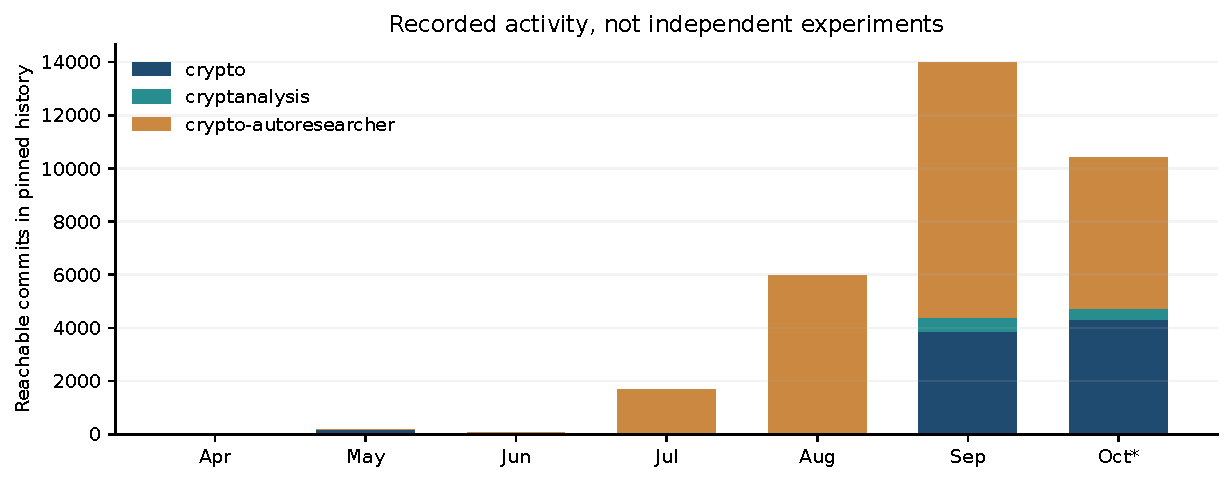
\includegraphics[width=\linewidth]{figures/activity.pdf}
\caption{Recorded activity in the three core pinned histories by
committer month. Merge and non-merge commits both occur in the histories.
Counts indicate archival volume, not independent experiments, researcher
hours, authorship, novelty or scientific success. October is partial.}
\label{fig:activity}
\end{figure}

\subsection{How the review was carried out}

The collection procedure used blobless Git histories, full tracked-tree
inventories, sparse content materialisation, repository indexes, ledger
parsing, and focused reads of studies and their code paths. The catalogue
contains 21,006 materialised Markdown documents under the documented size
and directory policy. A document's presence in that index means its title,
path and bytes were catalogued; it does not mean that every sentence was
manually assessed. A directory is similarly a navigational unit: several
directories can describe one study, while one directory can contain many
runs.

The 4,075 directory records cover \texttt{research/},
\texttt{experiments/}, \texttt{benchmarks/} and \texttt{papers/} across the
snapshots. The ledger catalogue parses 16,587 YAML files with a safe loader;
24 additional files could not be parsed by that loader and are retained
as explicit failures. Some root-level legacy records, archives and
checkpoints repeat or supersede other records. Record totals therefore
cannot be interpreted as distinct hypotheses or independent validations.
Both source paths and identifiers are retained so a reader can deduplicate
for a particular question.

The first synthesis used selective deep review. The subsequent request to
read everything prompted full-text reading of all fifteen root research
notes in the declared group, all twenty-one Markdown files in the pinned
ML tree, all nineteen ten-lead claim statements and all ten lead
descriptions. It also added complete reads of two implementation files and
two proof sources. These bounded completions do not complete the corpus.
The reading ledger records 94 fully read files (1,117,504 distinct bytes),
50 previously focused sources without complete reading receipts, and
305,223 entries without a reading receipt. Indexing, parsing and hashing
never count as reading. Appendix~\ref{app:reading} defines this boundary
and the unresolved exhaustive-reading obligation.

The review freshly checked byte hashes of all 19 frontier-session record
files, counted their outcomes, checked a downloaded volcano archive against
its complete manifest, and built the native C library and covered its
17 configured tests. Existing reports supply most experimental
measurements. The review did not rerun the full historical corpus, rent
accelerators, rebuild every Rust target, or rebuild Lean dependencies.
Every result below retains the distinction between source inspection,
fresh metadata verification, historical solver replay, and a new solver
execution.

\subsection{Access limits are part of the record}

The historical Autolab migration reports 186,032 files and
51,286,418,925 bytes across 32 task packages. Its 48-GB-class raw mirror is
a local working-tree archive, with manifests and materialisation receipts
in Git; it was not available as raw bytes in this runtime. Its structured
port comprises 84 historical EXP/RUN packages: 32 ALPF, 11 ALBIN, 38 ALISO
and three ALECF. These are archival claims with their original scope, not
freshly replayed results.\src{MIGRATION}

Likewise, the ten-lead advisory register preserves hashes and statements
for private source packets without including those packets. The public
register can be inspected, but full artifact replay cannot be inferred
from its structural validity. In contrast, the linked 37,926,124-byte
volcano checkpoint was accessible and was downloaded and checked. The
expanded search also located a later 73,208,632-byte, 7,937-vertex
checkpoint and a separate full-selected-point-order C diagnostic. Both
were downloaded and manifest-checked, without executing their binaries. These
are different access situations and are reported differently.\src{TEN}
\src{VOL-ARCHIVE}\src{VOL-V7}\src{VOL-C-FULL}

\subsection{A multidimensional assessment}

Progress has at least five observable dimensions: implemented capability,
verified correctness, lower cost on a fixed task, stronger experimental
instruments, and narrower uncertainty about a mechanism. The owner's
current criterion explicitly treats a verified improvement over the
current IC baseline as success, including constant-factor engineering.
Beating rho is a longer-term objective, not the admission criterion for
every useful implementation change.\src{C-RULES}

This paper accordingly preserves engineering gains even where IC remains
slower than rho. It also preserves negative results and corrections as
knowledge, while not counting them as speed improvements. A review verdict
such as ``ADVANCES'' in a study's local vocabulary is translated into its
actual boundary: a constant-factor improvement, a fitted exponent on a
bounded panel, a primitive saving, or an accounting correction.

The volume supports describing a substantial, highly instrumented
research programme. It does not support ranking the effort against all
human ECDLP research: comparable records of unpublished work, labour,
compute and independent scientific output are unavailable. This paper
therefore measures the accessible programme rather than asserting a
historical rank.

\subsection{Development over six months}

The first-parent history provides a useful chronology when interpreted as
provenance rather than proof. On 25 April, the initial educational library
was followed by known-answer tests and hardening work. Early May added
curve arithmetic, a broad attack taxonomy, binary curves, pairings,
summation-polynomial IC, cryptanalysis tooling and research benches. The
same period explored canonical lifts, Smart-style adaptations to
non-anomalous curves, $p$-adic constructions, coordinate correlations,
GLV/HNP ideas and geometric transfers. Several commit subjects use strong
phrases such as ``structural obstruction''; later revisions show why
those subjects must not be treated as permanent conclusions.

May--June Autolab work tested Howe gluing, Richelot and CM patterns,
GLV-related lattices, separator hypotheses and numerical behaviour. The
sequence includes a concrete example of progress through falsification:
successive proposed predictors of a lattice effect failed on expanded
cross-curve panels. The October LLL correction then withdrew a claimed
curve-specific failure after tracing it to floating-point behaviour,
including a diagnosis already present in the May numerical note.
\src{AUTOLOG}\src{HNP}\src{LLL}

July introduced the dedicated autoresearcher framework; the late-July and
August work imported historical experiments, built ledger and coordination
contracts, and expanded the research corpus. September concentrated on
Koblitz IC, SAT/F4 comparisons, invariant and compact-orbit bases, native
arithmetic and the independent cryptanalysis toolkit. October added
ecbench, more explicit cost accounting, root-finding oracles, field and
genus ladders, learning and symbolic discovery, large graph checkpoints,
equal-advice controls and shared Lean infrastructure. These stages
overlap: they describe development emphasis, not a sequence in which one
research direction replaced all the others.

\section{Mathematical setting and the field taxonomy}\label{sec:math}

The size of a field, the order of the whole curve group, and the order of
the subgroup containing the logarithm must remain separate. Throughout,
$q$ denotes a field cardinality, $r$ a prime subgroup order, $h$ a
cofactor, and $Q=[d]G$ a target in $\langle G\rangle$. A curve over an
83-bit field can contain a much smaller prime subgroup. Its ECDLP is
priced in that subgroup, not in the field size.

\subsection{Generic reference algorithms}

Pollard rho obtains a collision among combinations $[a]G+[b]Q$ and solves
the resulting scalar congruence. The familiar random-collision
normalisation is approximately $\sqrt{\pi r/2}$ group steps under idealised
assumptions. This is a model constant, not a universal implementation
bound. Negation, efficiently computable automorphisms, fruitless cycles,
distinguished-point density and restart policy change observed constants.
Parallel collision search changes throughput and coordination costs
without by itself changing the square-root exponent.\cite{pollard1978,vanoorschot1999}

Baby-step giant-step spends square-root memory to obtain another generic
tradeoff. Kangaroo is appropriate when the unknown scalar is known to lie
in an interval; its scale is the interval width, not automatically $r$.
Pohlig--Hellman decomposes composite orders, so a ``large curve'' whose
largest prime factor is small is not a large prime-order ECDLP instance.
These distinctions are implemented in the native toolkit and in the
challenge infrastructure.\src{CA-README}\src{COST}

Generic-group lower bounds establish asymptotic limitations under an
explicit oracle model. They should not be read as a sharp leading-constant
claim of exactly $\sqrt{r/2}$ operations for every implementation with free
negation. The cost challenge is valuable as an executable metering
instrument; this retrospective does not adopt every explanatory constant
in its README as a separately proved lower bound.

\subsection{Index calculus as a complete method}

Choose a factor base $\B=\{F_1,\ldots,F_B\}$, or a quotient of it under
known symmetries. A relation expresses a sampled point as a short sum of
base points. For example,
\[
 [a]G+[b]Q=\sum_i c_iF_i
 \quad\Longrightarrow\quad
 a+bd\equiv\sum_i c_i\log_G(F_i)\pmod r.
\]
After enough independent relations, linear algebra and a target descent
recover the logarithm. Relation count, matrix rank, and recovered scalars
are separate checks. A large number of valid but dependent rows can leave
the system unable to determine the requested target.

For a random-set heuristic with $B$ points and $m$ unordered summands, the
expected number of decompositions is roughly $B^m/(m!r)$. This is not a
universal yield theorem: repeated points, signs, orbit stabilisers,
cofactors, projection into $\langle G\rangle$ and collisions can change the
count. The programme repeatedly found that exact subgroup and base
conventions matter.\src{BOUNDARY}\src{HEUR}

Semaev's summation polynomials encode the existence of point sums through
their abscissae. They provide algebraic formulations, but replacing a group
problem by a polynomial system does not make the system cheap. The cost
of constructing, solving, lifting and verifying that system is central to
the programme.\cite{semaev2004}

\begin{table}[htbp]\small
\caption{Field and problem regimes in the portfolio. Evidence in one row
does not automatically transfer to another.}
\begin{tabularx}{\linewidth}{@{}p{2.7cm}YY@{}}\toprule
Regime & Structure used & Principal limitation in this record \\\midrule
$E(\F_p)$ & coordinate subsets, multiplicative towers, low-degree maps,
special endomorphisms & no general sub-rho prime-field IC demonstrated \\
Ordinary $E(\F_{2^n})$ & $\F_2$ subspaces, Weil restriction, Boolean
algebra & decomposition degree and total yield remain limiting \\
Koblitz $E/\F_2$ over $\F_{2^n}$ & Frobenius orbits and known subgroup
eigenvalues & rho receives the same available symmetry; setup is material \\
Composite-degree binary fields & proper subfields and GHS descent &
weak classes, genus and explicit maps determine applicability \\
Prime-degree binary extensions & no proper intermediate subfield &
composite-degree GHS conclusions require a new construction \\
$E(\F_{p^k})$, small fixed $k$ & base-field abscissae, Gaudry/Joux--Vitse,
torsion invariants & expensive algebraic constants and linear algebra \\
Higher-genus Jacobians & divisor arithmetic, covers, large primes &
source-subgroup transport and same-problem reference must be verified \\
Supersingular isogeny problems & graph navigation, quaternion and Kani
constructions & an isogeny problem or KEM is not the ordinary ECDLP \\\bottomrule
\end{tabularx}
\end{table}

\subsection{Prime, binary, and extension fields}

In a prime field, Frobenius exists but is the identity on field elements;
there is no proper intermediate subfield or nontrivial $\F_p$-linear
coordinate subspace. Saying that ``$\F_p$ has no Frobenius'' is therefore
an imprecise shorthand. The actual obstacle is the absence of a useful
nontrivial subfield decomposition of the kind available over extensions.
This does not rule out nonlinear sparse sets or other non-generic
algorithms.

In $\F_{2^n}$, an $\F_2$-subspace of dimension $\ell$ supplies a compact
membership condition for a factor base. Weil restriction turns an
extension-field polynomial into Boolean equations. The behaviour of the
resulting ideal depends on the formulation and product spaces, not merely
the nominal field degree. On Koblitz curves, the map
$\pi:(x,y)\mapsto(x^2,y^2)$ is also a curve endomorphism. Its action on the
selected cyclic subgroup can be represented by a known eigenvalue
$\lambda\bmod r$, allowing orbit-weighted relations.\cite{ggmp2020}

Over $\F_{p^k}$, a base defined by $x\in\F_p$ interacts with summation
polynomials through Weil restriction. Fixed-degree extension-field
algorithms and their symmetry reductions are established antecedents of
the implemented work. Their asymptotic opportunities do not imply
reasonable constants at the measured sizes, nor do they imply an
algorithm on $E(\F_p)$.\cite{gaudry2009,diem2011,fghr2014}

The implemented studies therefore cover prime fields, binary extensions,
and selected odd-characteristic extensions, notably degrees two through
six, together with protocol-specific extension arithmetic. This is not a
claim of a complete backend for every finite field, every characteristic
or every elliptic-curve model. Backend limits and unimplemented field
degrees remain separate from mathematical applicability.

\subsection{Isogenies and higher-dimensional transfers}

An isogeny defined over the working field is a homomorphism on rational
points. If its restriction to the prime subgroup is injective, then
$\varphi(Q)=[d]\varphi(G)$ preserves the logarithm. A destination solver
must still solve that transported instance more cheaply after charging
map discovery, construction, evaluation and recovery. A small degree,
shared $j$-invariant, common group order or common endomorphism field is
not by itself an executable transport certificate.

A cover or Jacobian route has more obligations: a concrete destination,
an explicit nonzero map, a proof or check of subgroup preservation, an
implementable destination solver, and the total source-to-answer cost.
Merely finding a low-genus curve with desirable arithmetic does not
establish that the source ECDLP can reach it. The portfolio's newer
identity and curve registries explicitly encode these distinctions.
\src{TRANSFER}\src{TEN}\src{VOLCANO}

\section{How the experiments measure progress}\label{sec:measurement}

The most consequential methodological change is the movement from a
headline counter to a complete, explicit accounting boundary. The same
research direction can look favourable when only relation probes are
counted, unfavourable when each probe is priced, and different again when
setup and linear algebra are included. The programme's rules were written
in response to concrete examples of this failure mode.\src{C-RULES}
\src{RESIDUAL}

\subsection{Cost boundaries and comparable units}

The historical normalisation is
\[
 S=\frac{\text{total charged group-addition-equivalent work}}{\sqrt r}.
\]
Within an explicit curve, subgroup and implementation, this makes a
square-root generic reference roughly flat. It does not make different
primitive weights, memory envelopes or target laws interchangeable. Some
studies count field multiplications, some Boolean word XORs, some
simulated instructions, and some admitted wall time. A conversion must be
measured or explicitly modelled before units can be joined.

A cold solve includes reusable setup, factor-base construction, indexes,
relation collection, matrix work, target work and verification. An online
solve starts after reusable state has been prepared and excludes that
state's construction. Both questions are useful. The online question
requires a comparator with the same advice and reuse opportunity; the
cold question requires setup on both arms. A ratio between IC cold
process time and rho online time can be recorded as a diagnostic, but is
not a matched cold method ratio.

The current one-target contract also separates target-dependent phases.
It disallows replacing a one-target rho reference with a multi-target
batch, or dividing a shared collision search by target count and calling
the result one-target latency. Repeated one-target workloads form a panel;
they do not become a single batch ECDLP simply because the statistics are
computed together.\src{C-RULES}\src{N83}

\subsection{Unpriced work and the sensitivity band}

Many historical counters omit native operations. Rho can omit
canonicalisations, partition hashes and table operations; IC can omit
root calls, native matrix work or membership tests. If $L_A\le C_A$ and
$L_B\le C_B$ are incomplete cost lower bounds, then $L_A/L_B$ does not
bound $C_A/C_B$ in either direction. A ratio of lower bounds is not a
lower bound on the ratio.

The October accounting rule therefore prices emitted unpriced operations
at several common weights, including $w\in\{0,0.1,1\}$ GAE, on all arms.
A ranking is accepted only if it survives the band. A missing counter
emission cannot be repaired by choosing a weight: it remains an
implementation gap. A pinned primitive calibration can supplement the
band but cannot silently replace it on one side only.\src{C-RULES}

The band is a sensitivity analysis, not a claim that a 64-bit XOR and a
hash-table lookup really have identical cost. This is especially visible
for F4: weighting every XOR at 0.1 GAE is much more expensive than one
study's pinned calibration near 0.002 GAE. The conservative conclusion
must state where it depends on the band or on a particular calibration.
\src{FRONTIER}

\subsection{From exploratory scripts to sealed records}

The record includes exploratory scripts, toy known-answer ladders,
Autolab tournaments, immutable experiment contracts, ICMS and ecbench
sessions, native compiler and emulator checks, hardware experiments,
and independent replay receipts. The ecbench instruments add explicit
specifications, method and workload identities, per-run outcomes, source
and binary hashes, host manifests, cost phases, replay audits and
comparison records. The SQLite index is a view of evidence, not a
substitute for the sealed evidence.

Earlier scripts remain useful historical observations. They do not
automatically meet newer isolation, primary-online-window or replay
contracts. In particular, the migration of a result into a dashboard
cannot improve its evidence tier. The research orchestrator likewise
separates an executor's observation from a coordinator's official status
transition and an independent review.\src{AR-README}\src{C-RULES}

\subsection{Controls and statistical design}

Several recurring practices are worth retaining: freeze the protocol
before the measurement; tune on disjoint training points; test on held-out
public points; interleave arms; include identical A/A controls; verify
every returned scalar or root set; retain failures; and bootstrap over the
actual independent workload or curve unit. Five targets are not 25
independent targets merely because five configurations ran on each.
Similarly, repeat-bootstrap intervals on one scalar panel do not become
coverage over arbitrary scalar distributions.

Positive controls show that an instrument can detect the proposed kind of
signal; null controls show whether the same apparent signal arises without
the mechanism. The ML studies use class-held-out splits and label
permutation; decomposition studies compare with exhaustive point sums;
GPU studies compare ranks and pinned variables across paths. A failed
control is retained even when the main result appears favourable.

Resource failures are a separate outcome. Exhaustion means the declared
search budget ended. A timeout or memory cap says something about the
specific execution, not nonexistence of the desired relation. A failed
artifact-integrity gate can make a run inadmissible without supplying
negative evidence about the mathematics.

\subsection{A freshly checked campaign}

The 15 October frontier campaign is a stronger common reference than a
collection of unrelated best cells. Its 19 sessions cover eight Koblitz
curves, six NIST-shaped prime curves and five prime Kummer-ladder curves,
with 16 public targets, two measured rounds and a warm-up. The sessions
contain 4,848 executions: 4,769 verified and 79 exhausted including
warm-ups. Removing warm-ups leaves 3,232 measured executions: 3,178
verified and 54 exhausted. Every stored record-file hash matches its
session manifest in this review. The stored audits contain 3,178
successful identical replays of verified measured records; exhausted
records are retained separately, not reported as successful replays.
\src{FRONTIER}\src{BAND}

No IC arm in that campaign beats the cheapest matched constant-memory
rho arm at any of the three band weights. Compact-orbit IC is closest on
the Koblitz ladder: its IC/rho ratio is 3.8--15.0 with the extra native
work priced at zero, and 4.9--17.8 at $w=0.1$. Prime pair-table IC grows
from approximately 10.5 to 101.8 times rho at $w=0.1$ over the
20--40-bit ladder. The campaign's fitted exponent differences are not
uniformly separated at every weight. This establishes a bounded
comparison on those implementations and instances, not a theorem that all
future IC must lose.

\begin{figure}[htbp]
\centering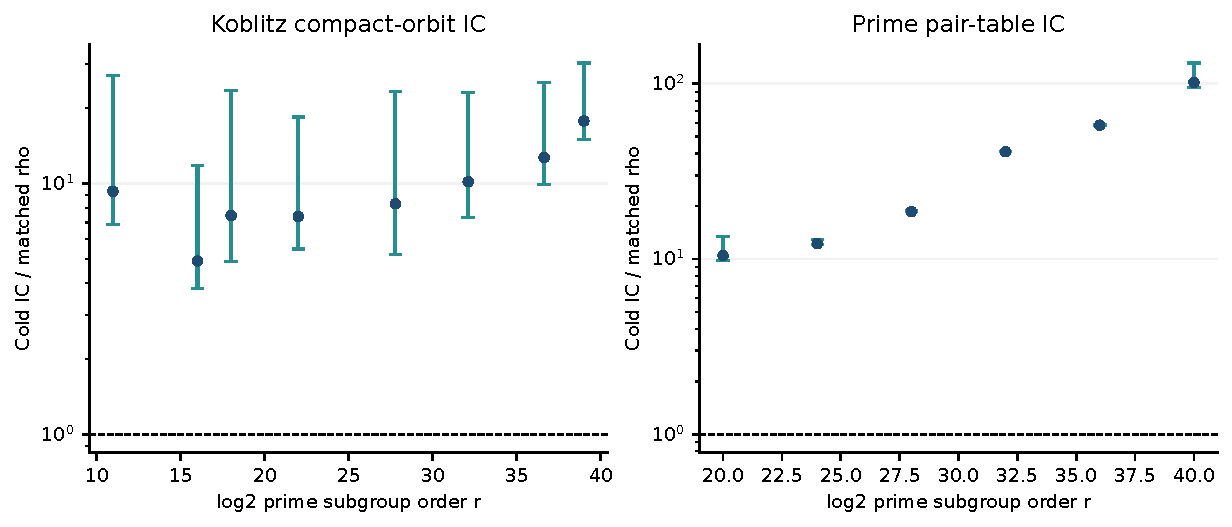
\includegraphics[width=\linewidth]{figures/frontier.pdf}
\caption{The campaign's recorded cold IC/rho ratios. The centre marks
$w=0.1$; the spans show $w=0$ through $w=1$. Every displayed cell has
32 verified measured runs. These are counted-work comparisons at L0,
not new native wall-time measurements. Koblitz points are ordered by
subgroup size, which need not follow field degree. Source: \src{BAND}.}
\label{fig:frontier}
\end{figure}

The campaign does not supersede every later experiment. Its role is a
fixed, comparatively well-accounted baseline. Later improvements require
their own matched comparison before being used to move this frontier.

\subsection{Corrections as an experimental capability}

The programme now has repeated examples of a result being made less
favourable by better accounting: a relation-only crossover disappearing
after linear algebra was priced, F6 geometry dominating its saved XORs,
and online IC losing an advantage after rho was given preprocessing.
These are scientific corrections. They are also evidence that the
instruments can reject a preferred interpretation. They should remain in
the record beside the successful optimisations rather than being removed
from a progress narrative.

\section{Prime-field research: sparse sets, root finding, and algebraic bases}\label{sec:prime}

Prime fields are the most demanding generalisation target in this
portfolio. Coordinate arithmetic is efficient, but the subfield
conditions used by extension-field IC are absent. The programme tests
several substitutes rather than treating this absence as a proof that no
alternative can exist.\src{PRIME}

\subsection{What the smallness experiments actually learned}

The dedicated smallness repository asks whether an inexpensive
coordinate-defined set behaves additively better than a matched random
set. Its experiments include intervals in $x$ and $y$, slopes, affine and
M\"obius images, Hamming weight, Farey heights, multiplicative subgroups,
random windows, Fourier spectra, low-degree polynomial sweeps,
Coppersmith constructions, Witt carries and learned log-bit predictors.
The main closure panel uses three roughly 20-bit prime-order toy curves.
\src{SMALL}

An illustrative observation is especially clear. For a base near size
2,048, ordinary coordinate predicates have pooled two-sum closure ratios
near one: $x<2048$ gives about 1.04, a subgroup predicate about 0.95, and
matched random sets about 0.98--1.00. A log-interval positive control,
which uses unavailable discrete-log information to define the set, gives
256.4 against a predicted 256.5. The control shows that the instrument
can see strong additive structure; the measured cheap predicates do not
show that structure on the tested panel.

The null comparison must match sign closure as well as cardinality.
Negation-closed sets have correlated pair sums, so a naive Poisson error
bar understates their spread. Random-window maxima must also be compared
with maxima from the same-size null search. The lesson is a concrete
experimental discipline, not a universal theorem that every inexpensive
predicate is random.

The Witt-carry and small-root studies examine why tempting analogues of
extension coordinates become expensive. Their polynomial degrees and
success thresholds belong to the specific constructions tested. A
failed learned log-bit predictor is similarly evidence about the models,
features, labels and curve sizes used. It does not prove that no
computational representation of prime-field structure can help.

\subsection{A useful reduction of the two-summand oracle}

For a short-Weierstrass model $y^2=x^3+ax+b$ in characteristic other
than two or three, and affine points $R,F$ with
$x_R\ne x_F$, the familiar chord formulas yield
\[
 S_3(x_R,x_F,X)=(x_R-x_F)^2
       \bigl(X-x(R+F)\bigr)\bigl(X-x(R-F)\bigr).
\]
Thus, once $F$ is fixed, the roots needed for two-summand decomposition
are already group-law expressions. One can subtract $F$ and test base
membership, handling signs and exceptional points explicitly, rather than
compute a fresh Gr\"obner basis. The proof source formalises the affine
algebraic identity; its coordinate definitions and hypotheses are visible
in the Lean file.\src{RF-PROOF}

This is an implementation opportunity, not a new general summation-law
theorem or a prime-field ECDLP breakthrough. The source audit explicitly
identifies prior sum-and-membership algorithms. It also corrects the
manuscript's broad lower-bound language: a reusable pair table can make a
repeated query constant-time after quadratic setup, so an unqualified
linear-per-query lower bound would be false.\src{RF-AUDIT}

The implementation family includes batched inversions for direct prime
subtraction, binary pair-sum tables, three- and four-summand meet-in-the-middle
variants, windowed scans, dense root indexes, Kummer-base variants and a
CUDA root-finding kernel. The prime and binary models use their own group
laws. The short-Weierstrass identity should not be silently substituted
for the generalized binary model $y^2+xy=x^3+ax^2+b$.\src{RF-PDP}
\src{RF-GPU}

\subsection{Measured improvements, with the comparator repaired}

The source audit reports binary per-decomposition ratios of 383 and
1,535 against matrix F4 at field degrees nine and thirteen. The
precomputed pair-table build is excluded from those query ratios. At
degree 23 a complete binary solve is reported 122 times faster with the
pair table, while F4 is faster at degrees five, nine and thirteen. This
reversal is evidence that setup and scale matter.\src{RF-AUDIT}

On five NIST P-curves the six-point-base query ratios are
3,021--5,802 against the benchmark's Buchberger implementation. The printed
benchmark label said ``F4'', but the timed source calls
\texttt{groebner\_f4::buchberger}. The corrected comparator belongs in
every reuse of those ratios. These experiments perform tiny-base oracle
work on large field parameters; they do not solve an unknown NIST-curve
logarithm.

The complete prime-DLP comparison against msolve has two evidence tiers.
At 16 bits, both totals are directly measured. At 20 and 24 bits, the F4
totals are composed from sampled per-query CPU cost and the root-finder's
measured query count. The reported factors of about 100, 105 and 50 must
not all be described as directly timed complete solves. Nor are any of
them comparisons against the strongest generic rho method.

The ecbench audit supplies a different view. On one registered 20-bit
prime subgroup, a pair table reduces the counted IC $S$ from 1,524.511 to
28.753 relative to direct subtraction. Its paired counted ratio is
0.018861. Native work remains unpriced on those prime arms, so that
quotient does not bound a complete-cost ratio. On a degree-17 Koblitz
instance, the corresponding IC comparison is fully priced in that
study's calibration: $356.894\to20.360$, paired ratio 0.057047. Even
there, the rho comparison has unpriced work and cannot be promoted into
a complete-cost speed claim.\src{RF-AUDIT}

\subsection{Kummer towers and the remaining algebraic question}

Petit--Kosters--Messeng-style bases use multiplicative and tower
structure to give summation systems more algebraic organisation.
\cite{pkm2016} In the recorded five-curve ecbench root-finding panel,
896 runs verify and the IC/rho ratios remain about 29--141. Changing a
plain base to a tower base of the same size changes that table-based
oracle's cost by roughly one percent. The conclusion is narrow: the
tower's algebraic structure is not exploited by that particular
enumeration/table mechanism. It says nothing decisive about a genuinely
algebraic tower solver.\src{PKM}

The large-memory work now addresses that distinction. At the pinned main
snapshot, several larger tower cells remain bounded or resource-limited.
An open branch subsequently records the $m=3,N=21$ run on a 124-GB,
32-vCPU host. Both targets finish all degree-seven reductions without a
refutation, then stop at the first degree-eight step under the frozen
dense-cap rule. The demanded $B'$ has 79,330,205,871 entries, approximately
317 GB at four bytes per entry; the recorded peak resident memory is
67.1 GB. The two runs take 6,445 and 6,416 seconds.\src{PR2160}

This is real execution progress relative to an unrun memory-gated card.
It does not supply a completed degree or a productive degree-eight
refutation. The branch's results explicitly leave the interpretation
between the protocol's inconclusive and lower-bound cases to the
coordinator. It would be inaccurate either to keep calling the cell
``never run'' or to call it a successful degree-eight solve.

Another open branch integrates prime tower F4, signature F5, an F6-style
closure and enumeration into ecbench. It reports 140 verified runs on
four 9--15-bit prime-order curves. F5 reduces the emitted F4 work on the
same trees, while F6's closures save essentially no total work. The
author-reported priced comparisons still favour enumeration and rho.
The first attempt is explicitly voided for thread-dependent replay.
These are unmerged engineering observations at their pinned PR head,
not an update silently applied to main's frontier.\src{PR2223}

\subsection{Earlier prime-curve structural work}

The May--August record also includes $p$-adic lifts, anomalous-curve
techniques applied outside their usual setting, CM analysis, GLV/HNP
lattices, twists and coordinate correlations. Its value includes
identifying which proposed bridge was absent. An efficient scalar
decomposition, a low-height coordinate or a numerical lattice anomaly
does not automatically yield an efficient unknown-scalar recovery
algorithm. The later LLL correction makes this especially tangible:
apparent differences between named curves can be implementation
artefacts.\src{HNP}\src{LLL}\src{STRUCTURAL}

\section{Ordinary binary and Koblitz research}\label{sec:binary}

\subsection{What the Koblitz structure buys}

The Frobenius-invariant base implementation checks invariance point by
point, folds columns into Frobenius orbits and carries the corresponding
known $\lambda^k$ weights into relations. Small-field records report
roughly degree-$n$ savings in relation bookkeeping and degree-$n^2$
savings in linear algebra, consistent with the known invariant-base
method. Rho also uses the available signed-Frobenius quotient, whose
idealised improvement is of square-root orbit size. Comparing IC to rho
without that available quotient would credit IC with a symmetry the
reference was unnecessarily denied.\src{KOBLITZ}\cite{ggmp2020}

The progression from invariant subspaces to divisor bases, SAT-optimised
bases, rank-guided constructions and compact signed-Frobenius orbit bases
is an important implementation record. The compact base stores orbit
representatives and their known scalar weights rather than an entire
quadratic pair table. It trades memory and rank-generation behaviour
against online probes. It is the closest IC family to rho in several
recorded small-curve comparisons, but its advantage relative to another
IC construction is not a claim that it beats matched rho.\src{COMPACT}
\src{FRONTIER}

\subsection{Correctness improvements underneath the speedups}

The September development record includes a consequential root-kernel
repair. A previous combined-inversion implementation treated equal or
zero abscissae as rootless, although the specialised $S_3$ equation becomes
linear or a square equation in those cases. Exceptional scans consequently
installed false nogoods. The repaired kernel handles those degeneracies;
its source includes exhaustive root-set comparison for all 16,384
abscissa pairs over $\F_{2^7}$ and larger-field checks through degree 53.
The historical degree-53 SAT example retains the same planted relation and
3,631 conflicts while removing 39,856 false nogoods. Pre-repair certificate
schemas fail closed rather than being silently accepted.\src{KOBLITZ}
\src{KOBLITZ-ARITH}

The same record repairs a nonmonic-pivot rank-tracker error. These are
correctness gains even when a headline solve time does not change.
Word arithmetic, batched inversions and cofactor projections then reduce
allocation and field-operation costs. The recorded Itoh--Tsujii schedule
uses seven rather than fifty-one multiplications at degree 53, but its
microbenchmark difference is below that host's timing noise. Lexicographic
SAT symmetry breaking increased conflicts and was left disabled. Such
rejected and inconclusive changes belong beside successful optimisations.
The source reads in this review are not fresh Rust test executions.
\src{KOBLITZ}\src{S3-COST}

\subsection{Production improvements that survive a narrow reading}

Free relations harvested from the root table are a concrete example of a
mechanism that is useful but smaller than first hoped. A degree-61 census
with 600 columns finds 147 nontrivial collisions but only 49 independent
relations against 599 required. The original predicted yield was about
60 times too high. That defeats the proposed large rank shortcut at the
tested construction; it does not make every free relation worthless.
\src{EQUAL}

The later production comparison tunes the baseline and candidate rather
than comparing a tuned candidate to an untuned incumbent. Its held-out
candidate/incumbent counted ratio is 0.960, with interval
[0.946,0.976], over 360 verified runs. The feature is on by default with
a switch restoring the previous path, and the study records exact A/A
behaviour. At the same fixed $K$, the degree-41 and degree-53 intervals
include one; degree 61's 0.962 remains the clean same-$K$ effect. The
earlier pooled 0.957 result is annotated not to be reused as the tuned
claim.\src{ROUND1}\src{ROUND2}

This is measurable, modest production engineering. It also illustrates
why ``a major lead did not produce its hoped-for yield'' and ``a useful
constant-factor improvement landed'' can both be true.

\subsection{N83: an exact cold-process example}

The five-point N83 holdout compares nearby compact-base sizes under a
frozen winner rule and Tier-1 cloud conditions. Its curve is
\texttt{icv1-f2m83-t6151469093347-9eba6cd5}, with model
$y^2+xy=x^3+x^2+1$, prime subgroup order
$r=8,569,786,107,849,059$ and cofactor 1,128,547,018.
The subgroup has about 53 bits; ``N83'' is the field degree, not an
83-bit prime-order subgroup.\src{N83}\src{N83-ROWS}

It is also a different model from the exact E0 degree-83 fidelity gate
in the repository contract: $y^2+xy=x^3+1$, subgroup order
2,417,851,639,230,796,216,685,689 and cofactor four. That E0 subgroup
has about 81 bits. The E1 holdout above is useful evidence for its own
workload, but matching field degree alone does not discharge that exact
E0/ECC2K-130 fidelity obligation.\src{C-RULES}

\begin{table}[htbp]\small
\caption{Recorded five-point cold-process means. The baseline's two
A/A child times are averaged per point before the panel mean. This is
a configuration comparison within IC, not a comparison of matched cold
IC and rho. Source: \src{N83-ROWS}.}
\begin{tabular}{@{}lrrrr@{}}\toprule
Columns & Usable points & Cold seconds & Setup seconds & Rank seconds \\\midrule
1,104 & 183,264 & 120.227 & 48.728 & 71.320 \\
1,108 & 183,928 & 121.296 & 48.955 & 72.171 \\
1,120 & 185,920 & 119.826 & 50.081 & 69.525 \\
1,152 & 191,232 & 122.471 & 53.067 & 69.255 \\\bottomrule
\end{tabular}
\end{table}

The 1,120-column arm saves 2.645 seconds over 1,152 columns, with paired
95\% interval [2.085,3.205] seconds. The 1,104-column arm saves 2.244
seconds, interval [1.980,2.508]. But the observed 0.401-second advantage
of 1,120 over 1,104 columns has interval [$-0.236$,1.038], so the frozen
selection remains \texttt{BOUNDED\_UNKNOWN} with no selected candidate
identifier. All 25 IC arms and five rho arms have recorded independent
replay, and the study retains five passing baseline A/A gates.

\begin{figure}[htbp]
\centering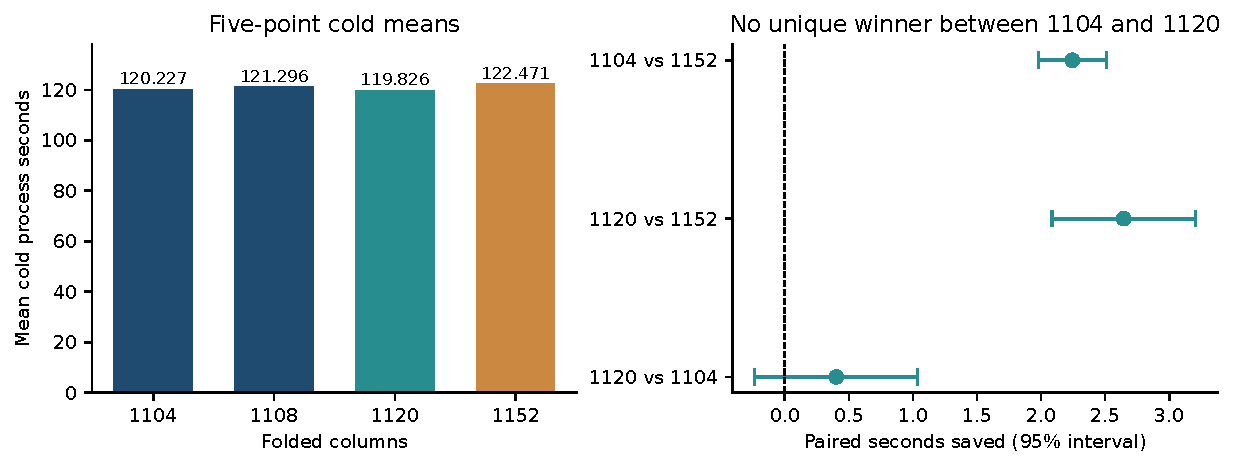
\includegraphics[width=\linewidth]{figures/n83.pdf}
\caption{A verified, held-out IC configuration improvement without an
overstated winner. Left: recorded cold-process means. Right: paired
seconds saved over the 1,152-column baseline, with the recorded 95\%
intervals; the final row compares the two leading candidates and includes
zero. Five public workloads, Tier-1 cloud instance. Source: \src{N83-ROWS}.}
\end{figure}

The setup/rank split identifies the next bottleneck more usefully than a
headline online ratio. Rank generation accounts for about 69--72 seconds
in these means, while target online work is a fraction of a second.
Reducing retained-state query latency alone cannot remove the cold rank
cost. Different base sizes also move the two phases in different
directions, which is why the winner rule should remain attached.

\subsection{Online ladders and the preprocessing control}

The historical ladder reaches degrees 53, 61, 71, 73 and 83, including
128-bit field packing beyond degree 64. The degree-61 two-host panel
records a 13.94 online rho/IC median ratio with interval [9.81,19.13]
on 64 fresh workloads, with roughly 28 seconds of setup excluded. These
are actual observations under that retained-preparation question.
\src{PRIOR}\src{COMPACT}

The equal-advice audit changes their interpretation. At degrees 41, 53
and 61, preprocessing rho uses the same or less retained advice and is
reported 53--317 times faster online by ratios of means; setup costs
are separately shown and are not matched in every such row. Some
controls fail their original prediction, and the host is contended.
Consequently the retrospective preserves the measurements, their
control caveats and their setup boundary, rather than treating them as
a universal dominance theorem.\src{EQUAL}

At degree 83, a later study runs time-matched and RSS-matched
Bernstein--Lange controls on 16 public points. Its K3300 time-matched
median IC/preprocessed-rho ratio is 3.74, interval [2.65,11.05]; its
RSS-matched ratio is 40.61, interval [24.27,71.72]. Its K600 comparisons
are larger. Under that protocol, neither original ``IC beats rho''
online interpretation survives matched preprocessing. The study also
states that no operation-count ranking is admitted: one band's order
flips, while another arm omits root-call emission.\src{EQUAL83}

The equal-bytes, single-process-group wide experiment at degrees 73
and 83 is nevertheless a distinct open requirement. Its instrument is
built and checked, but the frozen wide session is explicitly not run.
Time-matched and RSS-matched experiments should not be relabelled as
that missing experiment.\src{WIDE}

\subsection{Ordinary binary oracles and solving degree}

The ordinary-binary programme includes XOR-aware SAT, Semaev systems,
matrix F4, inherited F4, pair-and-solve oracles, meet-in-the-middle tables
and root finding. A binary MITM ladder reaches $\ell=12$, where the
recorded table has about 8.09 million sums and occupies about 259 MB.
The maximum counted query work is 16,092 point additions against about
8.39 million quartic solves in the comparator; witnesses and negative
answers are cross-checked on the panel. The table is target-independent
setup and is charged as such. The large query improvement is not an
end-to-end exponent improvement.\src{TIMELINE}

The degree-closure studies make another important distinction: plain
XL degree, first-fall degree, closure refutation degree and the cost of a
full Gröbner solve are not interchangeable. Full closure can refute a
system several degrees below an XL-only diagnostic. In the recorded
scale studies, two explanations survive the tested cells: a rise near
$\ell=7$, or a rise when $m\ell\ge21$. The $m=4,\ell=6$ cell separates
them and remains unmeasured at the required boundary. The sparse closure
is an independent correctness check on smaller instances, but is too
slow to resolve that boundary in the recorded experiment.\src{DREG}

For ECC2K-130, degree-five extrapolations are therefore optimistic
scenarios rather than measured cryptographic-scale solvers. The
reported $2^{71.13}$ row is in unconverted column-touch units, whereas
the $2^{60.81}$ rho figure is in group operations. A displayed
``10.32-bit gap'' is an arithmetic comparison of those model entries,
not a calibrated attack-cost ratio. Neither a memory failure nor the
absence of a favourable row proves a general lower bound on binary IC.
\src{DREG}\src{LEADS18}

\section{Algebraic engines, SAT, and linear algebra}\label{sec:solvers}

The solver programme is broader than a single F4 implementation. It
includes Boolean matrix F4, signature/F5 variants, inherited elimination
over assignment trees, geometry-assisted F6-IC, prime-field F4, tower
arithmetic, sparse and dense kernels, Four-Russians elimination, SAT/XOR
encodings, linear-row harvesting, GPU offload and destination matrix
solvers. These are reusable instruments, even where the current ECDLP
pipeline prefers an enumerative oracle.\src{GB}\src{CA-README}

\subsection{Inherited elimination and the accounting lesson}

Inherited F4 carries a parent's reduced information into a child partial
assignment rather than constructing a fresh Macaulay matrix at every
node. On the identical-tree K13 and random-13 panels, the record reports
matrix-work reductions of 198.6 and 222.1 relative to matrix F4. F5's
word-XOR ratios against F4 are about 0.6465 and 0.6414. These are
specific stage counters on particular systems, not a claim that every
F4 task is hundreds of times faster.\src{GB}\src{PRIOR}

F6-IC adds factor-base domain pruning and meet-in-the-middle leaves.
Its word-XOR count is lower than inherited F4, and its relation stage can
be faster. Once the leaf geometry and batched additions are charged,
however, the older complete-cost study reports F6-IC costs 64.6--68.8
times inherited F4 at degree 13 and 1,303--1,353 times at degree 19.
The saved algebraic counter moved work into another phase. That is an
accounting loss on those workloads, not a reason to delete the stage
measurement or to assume every future geometry-assisted engine must
lose.

The engine audit also found a prime-field soundness bug, contract
defects and latent holes. Its regression and brute-force comparisons are
part of the progress: a fast engine that can discard a real root is not
an acceptable oracle. Correctness must cover both positive witnesses and
negative decisions, not just the final answer on favourable targets.

\subsection{What the external comparisons establish}

The prime-field F4 work reports 29.8--54.1 improvements over its
predecessor on square generic systems, with msolve/ours ratios
0.96--1.22 in the recorded single-thread comparison. Reduced bases are
checked against external tools. This is a useful example of making the
external baseline explicit. It is not a comprehensive fastest-solver
claim over other degrees, fields, orderings, thread counts or hardware.
\src{FP-F4}

Task identity is equally important. Deciding whether a Boolean system
has an admissible root, extracting a few linear consequences, and
computing a complete reduced basis are different jobs. The fact that a
specialised oracle decides a target in milliseconds while a general CAS
spends seconds producing a full basis does not by itself establish a
corresponding engine speedup on equal outputs. The portfolio's newer
external-comparison rule requires the same inputs, outputs and host,
and names missing external tools rather than selecting a convenient
slower reference.\src{C-RULES}\src{PRIOR}

\subsection{GPU results: real acceleration and a negative deployment result}

The RTX 5090 experiment is particularly informative because it records
both. A degree-six Macaulay task with 168,363 rows and 188,203 columns
takes 425.8 seconds for host build plus elimination and 5.70 seconds for
device build plus elimination, a recorded factor of 74.7 on that pod.
Another degree-six matrix improves 25.5 times. Ranks, refutations and
pinned variables agree. The device column includes first-use CUDA/NVRTC
cost in the first elimination; separate upload and kernel times are also
reported.\src{F4-GPU}

Yet the small per-node device decider does not beat the production
inherited host engine. On its fixed 1,024-target oracle panel, the GPU
path takes 5.57 seconds while the default inherited host path takes
1.25 seconds. The GPU is useful on the large matrices; the better host
algorithm wins on the small repeated systems. A proposed deployment
should use this result to decide where to offload, rather than project
the large-matrix factor onto the whole IC pipeline.

The H100 follow-up records a kept tiled update, 1.11--1.49 times faster
on the measured matrices, and a reverted merged-basis panel that is
1.5--5.3 times slower. Upload costs remain. This is a concrete record of
an optimisation search with a retained unsuccessful arm.\src{F4-PANEL}

\begin{figure}[htbp]
\centering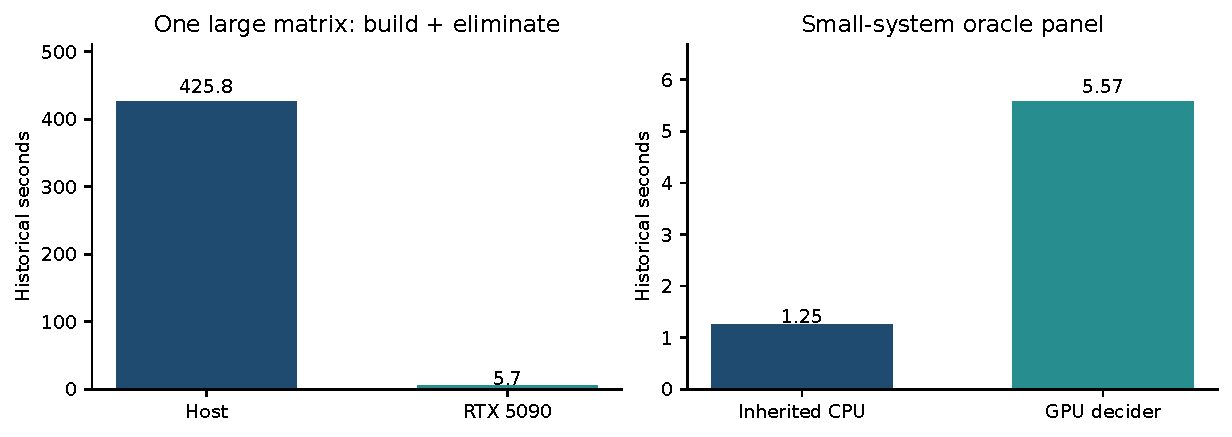
\includegraphics[width=\linewidth]{figures/gpu-stages.pdf}
\caption{Two different boundaries in the RTX 5090 study. Left: one large
degree-six matrix, host and device build plus elimination. Right: the
small-system oracle panel, where the inherited CPU engine is faster than
the GPU decider. Historical wall observations, not a new measurement or
an end-to-end ECDLP speedup. Source: \src{F4-GPU}.}
\end{figure}

The root-finding CUDA kernel is a separate case: the cited implementation
is host-emulated, with no GPU measurement in that study. Its validation
cannot inherit the F4 kernel's hardware evidence merely because both use
CUDA.\src{RF-GPU}

\subsection{Factor-base geometry and empirical solver selection}

The cryptanalysis product-profile study measures 656 factor bases from
seven families over nine fields. For two-summand systems it fits the
empirical rule
\[
 e=n-\dim V-\dim V^{(2)},\qquad
 D=2+[e<-3.5]+[e<-8.5],
\]
with mean absolute error 0.06 degrees, or 0.08 when leaving out each
field size. This is a fitted rule on that dataset, not a proved
degree law for growing parameters. In selected cells, geometric
progression bases reduce query cost 15--40 times relative to random
bases while leaving yield similar.\src{HEUR}

The three-summand comparison shows why formulation is another research
lever. Direct coordinates and symmetric variables live in different
product spaces. Minimising the dimensions of $V^{(k)}$ can reduce the
number of symmetric unknowns even at the same solving degree. The
report explicitly labels these rows PDP-stage profiles and keeps their
candidate identity unset until a calibrated complete pipeline exists.

It also identifies a practical stopping condition: a relation collector
can wait forever for full rank when the attainable matrix rank is one
less than the number of columns. Solving modulo the known kernel and
verifying the target is different from assuming that another dependent
row will repair it. This is a concrete lesson about implementations, not
only asymptotic analysis.

\subsection{Linear algebra and harvested information}

Linear algebra is the phase most likely to invalidate a relation-only
crossover. The residual-walk record documents a claimed relation-phase
crossing that disappears after matrix cost is included. Sparse filtering,
structured Gaussian elimination, Lanczos, Wiedemann and block Wiedemann
are therefore method components, not cleanup after the interesting part.
\src{RESIDUAL}

The later genus-three experiments compare complete solvers after changing
large-prime handling and matrix strategy. One structured-elimination and
Wiedemann route has recorded complete candidate/incumbent ratio 0.653
[0.647,0.660] at $q=2^{20}$, with 474 verified logs in its panel.
Its linear-algebra constant improves while the fitted exponent of that
phase rises. A subsequent block-Wiedemann change gives about 0.945 at
$2^{21}$; a combined schedule and solver reaches 0.605 of the earlier
round-one baseline. These factors belong to their named comparison
chains and are not multiplied into an invented cumulative factor on the
prime-field ECDLP.\src{ROUND2}

Linear-row harvesting is another modest, testable gain. The recorded
root-set panel has zero failures on 96 comparisons; selected oracle
cells improve about 1.07--1.17 times. The report also states where the
bench gain fails to carry into production because the production solve
stops at its first accepted root. The exact stopping policy is part of
the workload definition.

\section{Small extension fields and higher-genus pipelines}\label{sec:extension}

This work is where the programme most clearly explores known
non-generic asymptotic routes rather than trying to manufacture prime-field
structure. The results are interesting precisely because complete costs
can be measured against the same problem. They remain separate from
deployed prime-field curves and prime-degree binary challenges.

\subsection{The residual-walk and parity ledgers}

The $\F_{p^3}$ harness studies subspace factor bases, residual walks,
large primes, GLV symmetries, decomposition oracles and sparse matrices.
Its corrections show that an oracle that reduces the number of walked
residuals can make the method more expensive if the per-residual work
increases. One cited example reduces a headline walked count by around
two orders of magnitude while total cost worsens by about 4.6 times.
\src{RESIDUAL}

The same record prices linear algebra that earlier rounds omitted. The
linear-algebra growth then dominates a relation-phase exponent and
changes the claimed crossover. This provides an unusually concrete
negative result: the bottleneck is named and priced, rather than the
route being declared unsuccessful because it did not immediately beat
rho. The parity ledger extends this discipline to several degrees and
decomposition choices.\src{PARITY}

\subsection{Degree four: symmetry improves a real algebraic constant}

On suitable curves over $\F_{p^4}$, a rational two-torsion point and an
appropriate coordinate make the summation system invariant under a
$D_4$ action. The unweighted invariant formulation reduces a generic
4,096-dimensional quotient to 512. Its recorded decomposition constant
at $p=269$ is about $2.54\cdot10^{10}$ base-field multiplications,
approximately 48 times below the plain formulation.\src{PRIOR}

The weighted four-variable follow-up is stronger evidence of iteration
than quoting that original factor forever. It replaces the five-variable
presentation by invariants of weights $(2,2,2,1)$ and records a
3,979-row, 4,200-column matrix rather than the previous 13,412 by
11,628 matrix. At $p=269,1033,4093$, median counted costs are around
$1.4\cdot10^9$ multiplications including lift-back and reruns at the
next degree when required. This is roughly another 18 times below the
previous invariant formulation, and about 844--863 times below the
named plain reference at those primes.\src{D4}

The study keeps exceptions. At $p=17$, one of six planted targets is
degenerate; the other five agree with brute force and MITM. The nine
generic positive-control systems have the expected quotient dimension.
The gain is a decomposition-stage constant. The study explicitly does
not measure end-to-end $S$ for that weighted formulation.

Its crossover calculations are therefore model outputs. Earlier models
moved a degree-four handover from around $2^{150}$ to $2^{135}$; the
weighted follow-up reports a further handover near $2^{118.9}$ in its
particular model. Those are not three observed ECDLP crossings. They
depend on the relation rate, cofactor, matrix model, unit conversion and
the constant measured at much smaller sizes.\src{D4}\src{LEADS18}

The subsequent complete-method experiments also show that combining
individually attractive ideas need not help. A D4-plus-double-large-prime
variant makes linear algebra cheaper but total cost worse on its
held-out panel. Stopping at the first actual dependency then repairs
part of that loss: the later complete candidate/incumbent ratio is
0.979 [0.973,0.986] over 27 held-out curves. This is progress against the
incumbent, not a claim that the weighted stage and the complete variant
were one already-measured stack.\src{ROUND1}\src{ROUND2}

\subsection{Degree five: a large stage factor with a distant model crossing}

The quintic Joux--Vitse/torsion programme implements a four-point
decomposition test over $\F_{p^5}$. Its plain and Edwards-symmetry systems
have very different costs: the cited constants are roughly
$3.0\cdot10^{10}$ and $7.3\cdot10^7$ base-field multiplications, a
recorded stage factor around 416. But a corrected exact yield census
changes the residual rate from $1/(24p)$ to $1/(192p)$, worsening the
extrapolated crossover. A four-torsion follow-up then retracts an
anticipated degree-halving lever: the available translation does not
implement the needed involution over the stated base field, and the
measured saturation costs about as much as it gains in rate.
\src{QUINTIC}

These examples explain why a several-hundred-fold algebraic improvement
can coexist with an impractical complete-method prediction. The
programme has learned both a useful symmetry implementation and the
conditions under which its hoped-for scaling argument fails. Neither
observation should be compressed into simply ``torsion works'' or
``torsion does not work''.

\subsection{Covers and genus-three index calculus}

The cover programme implements extension fields, Cantor-style divisor
arithmetic, a GHS/Joux--Vitse-type cover, a point transfer and a
decomposition test checked against a separate enumeration oracle.
On the favourable weak class, reducing the oracle constant improves the
complete IC/rho ratio as size grows. It reproduces a known attack route;
the difficult additional question is whether a generic source can find
and reach such a class at a total cost below its own rho reference.
\src{COVER}

The more recent cubic-GHS/genus-three work adds double large primes and
new matrix strategies. The first improvement round reports a complete
cost exponent about 1.385 rather than 1.910 on a common
$q=2^{10}$--$2^{18}$ range. Earlier headlines compared different ranges
and are corrected. The candidate's local exponent rises at larger
sizes, so a global finite-range fit is not evidence that it has reached
the asymptotic $4/3$ prediction.\src{ROUND1}

A separately rebuilt genus-three baseline reports IC/rho around 0.252
at $q=2^{14}$ after the study's rho normalisation. That comparator is
rho on the same Jacobian subgroup, not rho on the original elliptic
curve before transport. The timeline explicitly labels it as a
Jacobian result. An ECDLP crossover requires the source transfer and
source reference to be in the comparison.\src{TIMELINE}

The later structured-elimination and block-Wiedemann rounds reduce
complete costs further, but also identify the relation phase and matrix
growth that remain. This is the strongest recorded fitted-exponent
improvement over an incumbent among the selected complete toy pipelines.
It is appropriately described as reproducing and engineering a known
higher-genus route at toy scale, not discovering a new exponent for
general prime-field ECDLP.\src{ROUND2}

\section{Isogenies, graphs, fibres, conductors, and transfer}\label{sec:isogenies}

The isogeny work is not a single failed shortcut. It contains several
different objects: explicit walks and map certificates, conductor and
endomorphism-ring calculations, fibre-aware bases, gluing and
higher-genus constructions, weak-node searches, graph-wide experiments,
and cryptographic scheme prototypes. Their obligations differ.

\subsection{What transport conserves}

For a homomorphism $\varphi:E(\F_q)\to E'(\F_q)$, let
$\kappa=\ker\varphi\cap E(\F_q)$. Suppose
$\B'\subset\varphi(E(\F_q))$ and take the complete rational pullback
$\B=\varphi^{-1}(\B')\cap E(\F_q)$. The recorded transport argument
states that the number of ordered $m$-decompositions of $R$ over $\B$
is $|\kappa|^{m-1}$ times the number of decompositions of $\varphi(R)$
over $\B'$. Each image tuple has $|\kappa|^m$ lifts, and exactly
$|\kappa|^{m-1}$ have the required sum.\src{TRANSFER}

This is a useful scoped statement. It applies to the declared
homomorphism and complete pullback domain. It does not prove that every
alternative factor-base geometry has the same cost, nor that every
non-homomorphic or higher-dimensional reduction is impossible. It
directs attention to three things that can still change: rational
kernel symmetry, destination geometry, and arithmetic/solver cost.
Map evaluation and source recovery remain additional costs.

Isogeny loops act as endomorphisms; on a fixed prime cyclic subgroup an
applicable endomorphism acts by a scalar. Faster evaluation can help
known-scalar multiplication or a generic walk. Turning it into a
non-generic unknown-log advantage requires another mechanism. The
portfolio correctly keeps these claims distinct in its newer transfer
and curve-identity rules.\src{FIBRES}\src{C-RULES}

\subsection{Conductor gaps and fibre-aware IC}

The conductor-gap programme examines whether endomorphism-ring levels
change the measured difficulty of a decomposition method. Two fixed CM
pairs with large prime gaps give recorded floor/crater counted-$S$
ratios 0.975 with 99\% interval [0.603,1.451] and 1.127 with interval
[0.922,1.342], across 192 verified records and 96 stored exact replays.
These observations do not resolve the general conductor-gap question;
they fail to detect an effect in those exact comparisons. Both sides'
unpriced work remains relevant.\src{CONDUCTOR}

Fibre closure and two-torsion symmetrisation can reduce redundant algebra
on a matched abscissa base. A later correction shows why the domain
must be specified: at matched column count, an apparent symmetry saving
can disappear. Similarly, the fibre-aware scaling panels improve a
specific method but show its IC/rho envelope widening with size at
fixed cofactor. The reported ratios rise roughly from 8--9 to 35--37
at cofactor four, and from 13--20 to 60--63 at cofactor 72.
\src{FIBRE-SCALE}\src{PRIOR}

The right question is therefore a controlled comparison on the same
transported target, base convention, subgroup and resource envelope.
Comparing two curves with different subgroup sizes or comparing an
orbit-redundant base to an already-quotiented base does not isolate
intrinsic hardness.

\subsection{The graph-building capability and its measured coverage}

The full-volcano work builds explicit finite graphs and routes, exports
explorers, verifies kernel maps, assigns conductor strata, and runs
bounded IC and generic solvers on selected vertices. This is a
substantial implemented capability. Graph generation, graph completeness
for a declared edge set, and graph-wide attack execution are three
different completion claims.\src{VOLCANO}

The accessible checkpoint covers three smaller classes with 24,823
declared vertices and 51 strata. The repaired checkpoint has 2,935
audited vertices: 989 in the mixed-conductor graph, 970 in the
three-power graph, and 976 in the two-power graph. All 51 strata have
samples. This is about 11.8\% of the declared vertex population,
not a completed graph-wide measurement.

\begin{table}[htbp]\small
\caption{Outcomes in the downloaded repaired checkpoint. They are
attempts across multiple arms and two target workloads per selected
vertex, not 46,960 independent curves. Source: \src{VOL-ARCHIVE}.}
\begin{tabular}{@{}lr@{}}\toprule
Quantity & Recorded count \\\midrule
Audited vertices / declared graph vertices & 2,935 / 24,823 \\
Strata sampled & 51 / 51 \\
Attempt records & 46,960 \\
Verified recoveries & 30,270 \\
Exhausted budgets & 14,626 \\
Timeouts & 2,064 \\
Relations found & 1,530,557 \\
Source relation trials & 74,829,850 \\
Actual decomposition calls & 71,296,000 \\
\bottomrule
\end{tabular}
\end{table}

Source trials and oracle calls differ because repeated queries can be
skipped before invoking the oracle. Timeout counters are unknown where
not emitted; they are not zero. Earlier report versions labelled source
trials as decompositions, and the corrected summary exposes both
denominators. Those corrections are a practical example of why raw
records and versioned summaries matter.

\begin{figure}[htbp]
\centering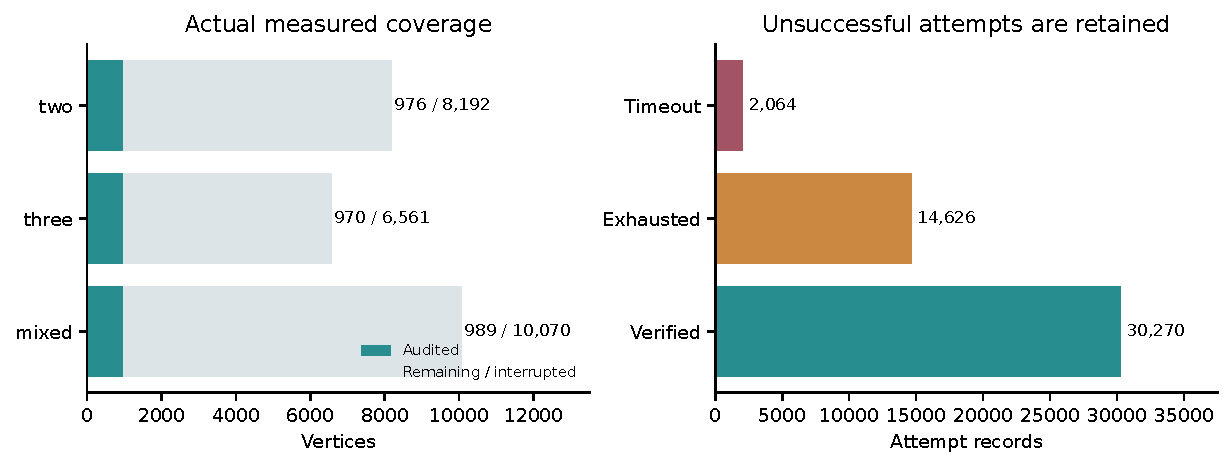
\includegraphics[width=\linewidth]{figures/volcano-coverage.pdf}
\caption{Coverage and outcomes of the actual 2,935-vertex checkpoint.
The left panel compares audited with remaining vertices in each of the
three finite graphs; the right panel preserves unsuccessful attempts.
This is a coverage chart, not an inference that unsampled vertices share
the same outcomes. All 51 strata are sampled. Source: \src{VOL-ARCHIVE}.}
\end{figure}

The three source models have very different largest prime subgroups:
61,751; 19,768,889,568,671; and 4,253. Their roughly 57--59-bit field
sizes must not be used as common subgroup security sizes. The original
A--E ambitions are much larger---about 7.83 billion expected vertices
and 515 strata---and remain separate incomplete work. The smaller
checkpoint cannot be described as completing those populations.

This review downloaded the archive and checked every one of its 29,409
manifest entries, with no missing entry or hash mismatch. That proves
byte consistency of this delivery. The checkpoint's solver audits are
same-implementation replays, not new independent validation by this
review. Its unqualified wall times and incomplete operation counts do
not establish a fastest-method or asymptotic claim.

\subsection{GHS mechanisms and the scope of a trapdoor demonstration}

The pinned main branch of \texttt{ghs-trapdoor} is a scaffold, but another
captured branch contains a Sage mechanism prototype. It describes a
composite-degree binary field $\F_{2^{20}}$ over $\F_{2^5}$, a weak curve,
an Artin--Schreier tower, a genus-four model, an explicit transfer, and a
small protected subgroup of order 7,717. The branch reports
homomorphism and subgroup-order checks, isogeny pullback, and end-to-end
toy ElGamal recovery.\src{GHS-MAIN}\src{GHS-BRANCH}

Those are mechanism claims on the branch, not a demonstrated scalable
escrow system. The toy destination solver is BSGS, whose square-root
cost is comparable to source rho at that tiny subgroup order. The
general claim that the public curve forces outsiders to use rho, or
that a secret chain is hard to replace with any useful public route,
requires additional analysis. Working-field ambiguity in the README's
Jacobian description also needs checking against the actual code and
certificates before a stronger transport claim is made. No fresh Sage
or Lean replay was performed here.

The distinction is especially important for ECC2K-130, whose extension
degree 131 is prime. A construction exploiting a degree-four extension
cannot simply be scaled by changing that parameter. The ten-lead
register contains finite order and map-class obstructions for particular
candidate Jacobians, but leaves other destinations and constructions
open.\src{TEN}

\subsection{What remains of the structural and hidden-route leads}

The structural-completeness draft organises seven families of known
isogeny/CM mechanisms. Its own correction now describes case-analysis
proof sketches that have not received independent review; an earlier
unconditional-proof sentence was removed. This paper therefore treats
it as an organised argument and source catalogue, not a proof that every
prime-field attack route has been exhausted.\src{STRUCTURAL}

A hypothetical hidden route should be assessed through separate
questions: mathematical existence, explicit construction, public
discoverability, subgroup action, destination advantage, evaluation and
recovery costs, and the availability of an equivalent public shortcut.
No inference about secret agency capability follows merely from a
large degree or a sparse weak class. Conversely, failing to make a
route practical in a toy study is not a proof of its universal
impossibility. These are the appropriate remaining obligations of the
programme's speculative endomorphism and isogeny leads.

\section{Learning, symbolic discovery, and experimental falsification}\label{sec:learning}

The ML repository is more than an attempt to predict secret scalars. It
implements curve and isogeny-class datasets, exact arithmetic features,
class-held-out learning, graph models, symbolic rule search, permutation
nulls, and certificate-producing follow-ups. Its useful outputs include
both rediscovery of planted structure and evidence that attractive
hardness correlations disappear under stronger controls.\src{ML}

\subsection{The hardness question after controlling for size}

The expanded M9 hardness report has 108,473 nodes in 377 isogeny classes,
over field sizes mainly 16--24 bits. It distinguishes the counted cost of
the C library's rho, an exact two-sum yield label, planted structural
labels, and within-class residual versions of those quantities. Whole
isogeny classes, field families and larger sizes can be held out.
\src{ML-HARD}

A large global $R^2$ is not evidence of a new hardness predictor. For
plain-rho cost on the isogeny-class split, the full model's $R^2$ is
0.884 while the ceiling-only baseline is 0.885. For negation-rho it is
0.864 against 0.863, with a skill interval including zero. Much of the
global predictability is the known size and automorphism law. On
within-class blind cost labels, the added skill is essentially zero or
negative in the reported panels.

The positive controls do work. The within-class planted-rho label has
$R^2=0.914$ for the planted-safe model against 0.918 for its oracle;
other planted folds are recovered strongly. Thus the experiment can
detect a deliberately supplied structural law. It does not find a
corresponding blind law that improves the measured IC pipeline.

\begin{figure}[htbp]
\centering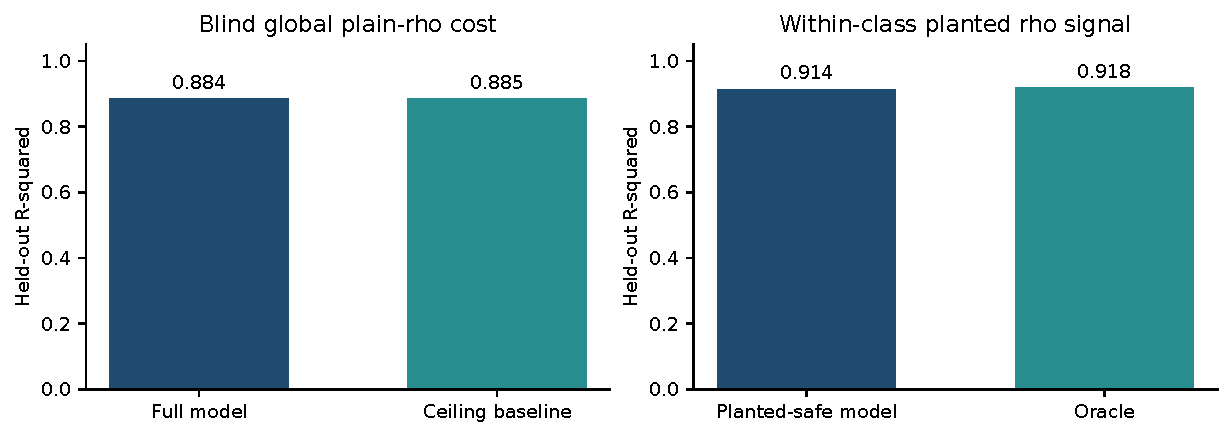
\includegraphics[width=\linewidth]{figures/ml-controls.pdf}
\caption{Why a high prediction score alone is insufficient. Left:
global plain-rho cost is already predicted by the simple ceiling
baseline. Right: a within-class planted structural control is recovered
near its oracle. These are different labels and are not a comparison of
two attack speeds. Recorded M9 values on the isogeny-class split;
source: \src{ML-HARD}.}
\end{figure}

The report also exposes power, split design and feature leakage. A model
using walk-sampling features can learn which node was planted as a root
rather than a transferable mathematical property. A learned policy must
eventually be charged for features, inference, selection and missed
solutions inside a held-out complete pipeline. No such learned component
is shown here to improve the current measured IC frontier.

\subsection{Binary GHS labels vary, but they are formula labels}

The GHS study covers 507 classes and 114,453 nodes over fourteen fields.
It computes exact structural invariants and applies a declared
literature cost formula. The descent label varies within isogeny classes
through the curve coefficient; planted weak nodes and subfield-type
structure are not the same phenomenon.\src{ML-GHS}

On held-out classes, coefficient invariants identify the weak-node label
much better than intrinsic graph features: reported in-class AUCs are
about 0.98 and 0.60. The subfield-degree/endomorphism-level relation has
zero violations on 99,269 checked nodes in the report. These are useful
structural observations and tests of a formula model. They are not
measured complete GHS attack times, and they do not establish a
secret-to-public discovery asymmetry at cryptographic scale.

\subsection{Extension-field degree measurements}

The $\F_{p^n}$ study covers 453 curves over degree-two and degree-three
extensions, with random, subfield, twist, isomorphic and isogenous
families. Its 5,592 target/system rows have Macaulay ranks equal to the
reported regular-sequence values, with the stated solving and
refutation-degree behaviour. It finds target-level degeneracy and
model-over-subfield effects, rather than a general lower degree from
sharing an isogeny class.\src{ML-FPN}

This is evidence about particular formulations over the tested primes.
It should not be pooled with Boolean first-fall experiments as if they
measured the same ideal or the same degree. It also explains why
``isogenous'' and ``same decomposition geometry'' must be distinct
features in a predictive experiment.

\subsection{Symbolic discovery with exact follow-up}

The Smith genus-three programme constructs and studies rational
$(2,2,2)$-isogeny mechanisms on 140,000 random squarefree octics. Its
observed density of curves admitting the declared rational isogeny is
0.1864, with interval [0.1843,0.1884], near the cited prediction 0.1857.
It separately tests trigonal-map rationality, isogeny rationality and
independence across pairings.\src{ML-SMITH}

The rule miner searches products of explicit quadratic-character
features and evaluates candidates on held-out primes and label
permutations. The follow-up twist-bit report has 5,811 certified
nondegenerate cases with no counterexample to the stated character law;
266 trace-zero cases are explicitly not certified by that point-count
criterion. Algebraic identities are checked on additional large-prime
panels. This is much stronger than reporting a classifier score, because
it produces a readable candidate rule and a certificate boundary.
Finite validation remains distinct from a proof for all permitted
curves.\src{ML-TWIST}

The Humbert-surface work recovers equations for $H_4,H_5,H_8,H_{12},H_{13}$
from structured source points, checks them against published equations,
and tests fresh primes. The recorded least weights are 30, 24, 60, 120
and 120 in the chosen invariant presentation. This is a successful
rediscovery and validation workflow, not a priority claim for new
Humbert equations. It also corrects an overgeneralisation: rational real
multiplication in a particular family cannot be inferred for every
point of a Humbert surface from the residue symbol $(D/p)$ alone.
\src{ML-HUMBERT}

\subsection{Assessment of the learning leads}

The most useful learning output so far is an instrument for generating
explicit, falsifiable structural candidates and then removing leakage
and simple explanations. The main hardness-prediction result is
negative beyond the known baselines at the measured scale; the symbolic
and planted-control results are positive within their declared tasks.
Future learning should target a concrete complete-method decision, such
as a base or solver policy whose feature cost is charged, rather than a
large global $R^2$ with no effect on ECDLP work.

\section{What was built around the mathematics}\label{sec:systems}

\subsection{A portfolio of executable instruments}

The Rust library implements field and curve arithmetic, generic and
specialised discrete-log methods, factor bases, Semaev oracles, SAT and
matrix engines, transfer experiments, external-CAS exporters, cost
accounting, curve identity and visual tools. The native C library
provides 64-bit reference groups and solvers, statistics, batched curve
arithmetic, preprocessing, bindings and distributed interfaces. These
64-bit primitives are research instruments; their parameter limit is
not a claim of cryptographic-size support.\src{C-README}\src{CA-README}

The broader library also contains symmetric ciphers, hash functions,
signature and nonce demonstrations, RSA and factoring routines,
pairings, zero-knowledge examples and post-quantum educational
implementations. Their presence documents capability breadth, not an
audited production cryptographic stack. For example, the current README
explicitly labels the STARK-like modules as educational, unaudited and
unsuitable for supporting a research security claim. This review does
not turn a module inventory into a security certification.

WDSat and the SQIsign repository are upstream solver/protocol forks and
integration resources; their imported histories are not independent
algorithmic contributions by this programme. The small standalone
ecbench repository is a companion entry point, while the principal
measuring implementation lives in crypto. Isogeny-labs supplies a
presentation layer. FPGA work includes field, point, step-unit and walker
models and simulation targets; the code inventory alone establishes no
measured silicon throughput. These distinctions prevent repository
proliferation from being counted as an equivalent number of new solvers.
\src{C-README}\src{CA-README}

The generic-group cost challenge adds a particularly useful boundary:
the solver receives opaque point tokens, while an oracle owns the real
coordinates and operation counter. This prevents an implementation from
silently doing unmetered point arithmetic. The same discipline motivates
the later explicit counters and sealed session records, although a
coordinate-aware IC study is a different computational model.
\src{COST}

\begin{figure}[htbp]
\centering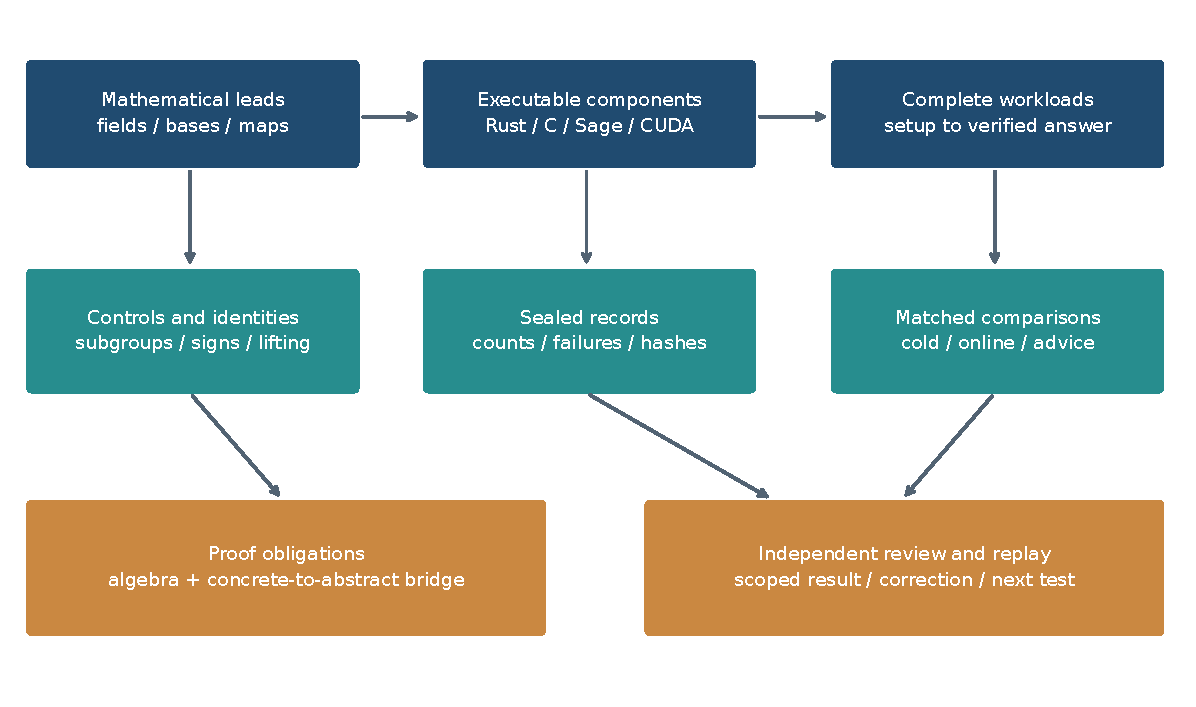
\includegraphics[width=\linewidth]{figures/research-map.pdf}
\caption{The implemented research stack and the distinct obligations
between a mathematical lead and an accepted complete-method claim.
Arrows are a conceptual workflow, not an assertion that every historical
study passed every gate. The catalogue and source register link the
concrete implementations behind each box.}
\end{figure}

\subsection{Research automation and preservation}

The autoresearcher separates coordinator, idea generator, executor,
reviewer, validator and red-team responsibilities. It implements
protocols, role policies, handoffs, immutable records, archive receipts,
corrections, claims, knowledge retrieval, runbooks and resource
coordination. This is research infrastructure whose aim is to prevent
an observation from being mistaken for an official scientific
transition.\src{AR-README}

The freshly parsed direct \texttt{ledger/goals/} files contain 72 goal
records: 36 draft, 26 active, six completed and four closed at budget.
These are literal stored status fields, not this paper's judgement of
scientific completion. Direct hypothesis files include 2,124 parsed
records; only 32 have exactly the literal status \texttt{supported}.
Other scoped and custom statuses are retained in the catalogue rather
than forced into a binary success metric. Legacy root records account
for why a whole-ledger wrapper count gives different totals.

The direct directories also contain 6,256 parsed handoffs, 2,634
proposals and 187 questions; missing status fields are common. These
counts measure coordination volume. Without deduplicated chains from
proposal to execution to independent review, they cannot yield a
meaningful ``research success rate''. The 24 safe-loader failures and
explicit correction records identify maintenance work rather than
silently disappearing from the denominator.

Cairn and associated runtime tools provide execution and custody
coordination. Their source and commits belong in an implementation
assessment, but this review does not infer actual rented compute,
financial spend, agent-hours or effective parallelism from their
existence. No verified consolidated bill or complete compute ledger
was available for that purpose.

\subsection{GPU rho, CPU arithmetic, and challenge operations}

The Blackwell release records an audited campaign build at 14.64
billion rho iterations per second on an RTX PRO 6000 Blackwell, with a
later best build at 15.88 billion. Its central mechanism is accelerated
binary-field arithmetic using the carry-less multiplication exposed by
the cited CUDA/PTX toolchain. Those are historical hardware-throughput
claims with provenance to the three central repositories; this review
does not remeasure them.\src{RHO-GPU}

The README also distinguishes the developed measurements from the
release snapshot's validation: the CPU client and planted solves were
run from that copy, while its Docker image and GPU modes were not yet
run there. The multi-card completion times are estimates from a work
model, not completed ECC2K-130 recoveries. Different documents quote
roughly 4.3 or five card-years under different builds and constants;
they must retain those assumptions rather than become a single measured
campaign duration.

The \texttt{ecc-challenges} service adds an operational evidence chain:
versioned raw uploads, namespaces, admission receipts, record validation,
point-relation checks, indexing and collision recovery. A durable upload
ACK is not the same as verified work. The v2 path checks curve membership
and $R=[a]G+[b]Q$ before index insertion, while reported trail lengths
still lack a work-verification model. Consequently point counts and
upload volume cannot honestly become percentage completion of a
challenge.\src{ECC-SERVICE}

An open C-library branch also identifies fruitless cycles in the GLV
walk and reports a corrective implementation. Its paired operation
ratios are 0.658 for $j=1728$ and 0.768 for $j=0$, with Bonferroni-adjusted
98.75\% intervals [0.630,0.688] and [0.753,0.784]. The author reports
432,000 correct toy solves across three builds. These are unmerged,
operation-count observations on 24--32-bit subgroups; the change does
not prove a new ECDLP hardness law. A stronger generic implementation
also changes the reference against which future IC must be measured.
\src{PR953}

\subsection{Quantum circuits and scheme construction}

The quantum point-addition work log studies reversible arithmetic scored
by average Toffoli count times peak qubits. Its recorded baseline is
1,739,149 average Toffolis, 1,434 qubits and score 2,493,939,666 over
9,024 validation shots. It also records truncation and reroll screening.
Those observations concern simulated circuit resources and finite
validation. Adaptive screening for a favourable Fiat--Shamir test set
does not prove correctness on every input. Upstream challenge progress
must not be credited as this programme's independent circuit advance,
and no fault-tolerant hardware ECDLP execution is demonstrated.
\src{QUANTUM}

EigenX is a separate constructive output: a Rust KEM/PKE research
implementation, wire formats, parameter sets, known-answer and hostile
input tests, and a Kani-chain/endomorphism design. Its current README
separates classical-optimised and quantum-hardened claim tiers after a
correction to earlier category language. Correct decapsulation at the
nominal parameter sizes establishes functionality, not the conjectured
security level. This is a scheme-construction research line and is not
evidence of an ordinary ECDLP break.\src{EIGEN}

Finally, \texttt{cryptologic-archives} preserves international standards
and historical cryptologic sources with claim and source catalogues.
It contributes provenance and contextual research, while its documentary
counts are not algebraic ECDLP experiments.\src{ARCHIVES}

\section{What is proved, observed, conditional, or still unproved}\label{sec:proofs}

\subsection{A proof map with explicit bridges}

The portfolio has moved from isolated Lean files toward a shared
\texttt{CryptoLean} library and a repository-wide proof gate. The shared
library pins Lean 4.35.0 and a Mathlib revision; historical dependency-free
projects can use other pins, such as the scoped torsion workspace's
4.22.0. A blanket statement that every proof uses one verified toolchain
would therefore be incorrect.\src{LEAN}\src{TORSION}

The gate builds targets and audits transitive axioms, accepting standard
foundations and rejecting \texttt{sorryAx}, unlisted native evaluation and
user axioms. Its README correctly states that passing this gate does
not establish that the formal theorem is the report's theorem. A faithful
mathematical bridge and an independent statement review remain needed.
This review inspected central proof sources and receipts, but did not
run a fresh Lean kernel build; it does not issue a new kernel certificate.

\begin{longtable}{@{}p{3cm}p{5cm}p{5.4cm}@{}}\toprule
Result or argument & Supported statement & Remaining boundary \\\midrule\endhead
Semaev $S_3$ roots & The committed Lean source proves the displayed
affine algebraic factorisation and root equivalence under curve equations
and distinct abscissae. & Coordinate/chord definitions are visible; exceptional
points and the relevant curve-model interpretation still belong to the
implementation contract. No fresh kernel build here. \src{RF-PROOF} \\
Odd-torsion translation & Under the stated additive laws, odd $r$,
$[r]P=0$ and nonzero two-torsion $T$ imply $[r](P+T)=T\ne0$. & The new
generic proof is distinct from the imported curve application. No concrete
point model or factor-base membership checker is imported by that file.
\src{TORSION} \\
Transport conservation & A homomorphism with a complete rational-pullback
base has the stated kernel-fibre decomposition count. & It is a scoped
written argument, not a new audited Lean theorem here or an exclusion of
all different bases and reductions. \src{TRANSFER} \\
Coprime group orders & A homomorphism between finite groups of coprime
orders has trivial image; the register applies a finite order check to
named source/destination pairs. & It excludes those homomorphism routes,
not every higher-genus destination or every reduction. \src{TEN} \\
Smith/twist and Humbert laws & Explicit identities, published-equation
comparisons and finite certificates support the stated populations. &
Zero finite counterexamples and a checked interpolation do not alone prove
every global mathematical extension. \src{ML-TWIST}\src{ML-HUMBERT} \\
Structural completeness & A seven-family taxonomy and case-analysis
proof sketches with an explicit October correction. & Independent review
and stronger proofs remain due; no universal security theorem is
established. \src{STRUCTURAL} \\
Degree plateaus and exponent fits & Exact outcomes on frozen bounded
systems; fitted exponents on named size ranges. & No proved global degree
law or cryptographic-scale asymptotic improvement. \src{DREG}\src{FRONTIER} \\\bottomrule
\end{longtable}

The shared library itself lists unfinished bridges, including the
relation between its concrete binary-polynomial computation and the
Mathlib polynomial object, group-level isogeny and generic-group
definitions, and additional Semaev/degree material. These omissions are
explicit research obligations, not proof failures to hide.\src{LEAN}

\subsection{Corrections that change the scientific reading}

\begin{enumerate}
\item \textbf{A solver label was wrong.} The several-thousand-fold NIST
query ratios are against Buchberger, not the claimed F4 comparator.
The large effect remains a stage observation with the corrected label.
\src{RF-AUDIT}
\item \textbf{A complete-solve label hid composition.} The larger prime
msolve totals were composed estimates from sampled per-query cost, unlike
the directly timed 16-bit comparison.\src{RF-AUDIT}
\item \textbf{Unpriced algebra changed the ranking.} F4 XORs and F6
geometry can dominate cost after being included. A lower algebraic
counter is not a lower total.\src{GB}\src{C-RULES}
\item \textbf{Online preparation changed the comparator.} The historical
IC online ratios remain observations, but matched preprocessing rho
removes the claimed advantage under the later controls. The exact wide
equal-bytes protocol is still distinct and unrun.\src{EQUAL}\src{EQUAL83}\src{WIDE}
\item \textbf{Relation count was not rank.} The free-collision census
finds far fewer independent rows than collision counts suggest. A later
tuned production improvement survives on a smaller constant boundary.
\src{EQUAL}\src{ROUND2}
\item \textbf{A trace-zero control sampled the wrong population.} The
apparent 50\% rejection does not apply to the production odd-order IC
targets. The integrated filter makes zero rejections in 29,624 checks
and contributes no such gain.\src{ROUND1}
\item \textbf{LLL failures were misattributed.} The corrected note
withdraws curve-specificity and identifies floating-point overflow for
the relevant cases. It also withdraws an unsupported P-521 mechanism:
the fixed-point recovery stands, but the scaled-floating failure's exact
cause remains unresolved. Repeated deterministic probes are not distinct
instances.\src{LLL}
\item \textbf{The structural proof was overstated.} The manuscript now
admits proof sketches rather than an independently reviewed unconditional
theorem.\src{STRUCTURAL}
\item \textbf{An Semaev expression defect may affect historical results.}
An open matched legacy/repaired rerun is designed around the archived
call sites. Some trial packages exist; the final validation and ledger
transition are not complete in the observed PR snapshot. Older exposed
results remain integrity-qualified until that audit resolves them.
\src{PR2412}
\item \textbf{A simulated campaign is not a measured one.} The open
synthetic-volcano PR explicitly labels its 130,410 observations as
invented cost-model records with no actual curves or recovered logs.
It is useful planning and presentation tooling and is excluded from
this paper's empirical attempt counts.\src{PR2236}
\end{enumerate}

These corrections should remain searchable beside their original
claims. Suppressing superseded evidence would make future reviewers
repeat the same misinterpretations. Conversely, a correction does not
erase a separately valid measured improvement whose boundary was never
the corrected one.

\subsection{What the combined record does not prove}

No inspected evidence establishes a general classical prime-field
ECDLP algorithm with exponent below one half, a cryptographic-scale IC
solution of ECC2K-130, or a method that recovers a standard deployed
curve's arbitrary unknown logarithm from the public point alone. The
record also does not prove the security of those curves or the
impossibility of a future non-generic attack. Generic-model bounds,
finite search failures, component improvements and implementation
limits have different logical force and must not be substituted for
one another.

\section{Lead assessment and the next discriminating work}\label{sec:assessment}

\subsection{A concrete progress ledger}

The table below collects examples that answer ``what improved?'' without
collapsing unlike tasks into a single progress score. Ratios are
candidate/incumbent unless explicitly stated otherwise. A value below one
means less of the stated cost, not necessarily a faster complete ECDLP.
No cumulative factor is obtained by multiplying rows with different
inputs, baselines or boundaries.

\begin{longtable}{@{}p{3.7cm}p{3.1cm}p{3.5cm}p{3.1cm}@{}}\toprule
Concrete change & Recorded progress & Boundary and evidence & Remaining limit \\\midrule\endhead
Production free relations & 0.960 [0.946,0.976]; 360 verified runs &
Tuned complete counted IC comparison; engineering. \src{ROUND2} &
Small gain; not a sub-rho result \\
N83 smaller compact base & 2.645 s saved [2.085,3.205] & Five-point
cold-process holdout; engineering. \src{N83} & Two leading candidates
not significantly separated \\
Weighted D4 solver & About 18 times less than previous invariant form &
Decomposition constant, several primes, root checks; engineering.
\src{D4} & No complete-method $S$ in that study \\
D4 first-dependency stop & 0.979 [0.973,0.986] & Complete counted
comparison on 27 held-out curves. \src{ROUND2} & Extension-field toy regime \\
Genus-three matrix route & 0.653 [0.647,0.660] at $2^{20}$ & Complete
counted solve; 474 logs verified. \src{ROUND2} & Phase exponents and
source-to-Jacobian comparison remain distinct \\
F4 large matrix on RTX 5090 & 425.8 s to 5.70 s & Same task, ranks,
refutations and pinned variables. \src{F4-GPU} & Stage only; inherited
CPU wins another oracle boundary \\
H100 tiled update & 1.11--1.49 times faster & Historical device-stage
measurement; engineering. \src{F4-PANEL} & Upload and full-query costs remain \\
Inherited F4 & 198.6--222.1 times less matrix work & Identical-tree
stage comparison. \src{GB} & Not a uniform general-CAS speed claim \\
Factor-base degree predictor & MAE 0.06; 0.08 leaving out fields &
Empirical rule on 656 bases. \src{HEUR} & Not a proved scaling law \\
Symbolic twist-bit rule & 5,811 certified cases, zero counterexamples &
Finite certificate-backed observation. \src{ML-TWIST} & Global theorem
and independent semantic review are separate \\
Graph-wide instrument & 2,935 audited vertices, 46,960 attempts &
Actual checkpoint; manifest freshly checked. \src{VOL-ARCHIVE} &
11.8\% of declared smaller graph population \\
Native-toolkit reproducibility & 17 configured tests covered & Fresh
Release build, 15 initial passes plus two repaired-environment passes &
Core native tests, not every historical experiment \\\bottomrule
\end{longtable}

\begin{figure}[htbp]
\centering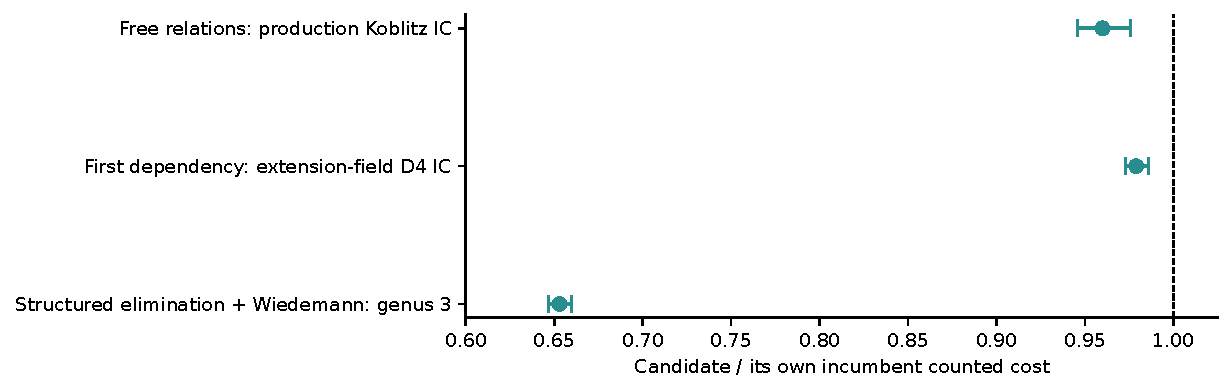
\includegraphics[width=\linewidth]{figures/incumbent-improvements.pdf}
\caption{Selected recorded candidate/incumbent comparisons. Each row
keeps its own task and baseline: the chart is a compact ledger, not a
ranking of methods or a cumulative speedup. Intervals are those reported
by the underlying studies. Sources: \src{ROUND2}.}
\end{figure}

These examples support four concrete conclusions. The programme has
built working instruments rather than only speculative notes. It has
made verified improvements over its own IC incumbents. It has developed
stronger controls that reverse some attractive interpretations. And it
still has a measured gap between its complete IC methods and the
strongest matched generic reference in the principal cold campaign.

\subsection{The ten open leads, without blanket closure}

The public ten-lead register preserves nineteen advisory records. Every
lead remains open in that register and no official hypothesis status is
changed by this paper. The observations below are what the register
reports; its private supporting packets were not freshly replayed here.
The proposed next steps are discriminating tests, not scheduled runs or
completed experiments.\src{TEN}

\begin{longtable}{@{}p{3.1cm}p{5.5cm}p{4.8cm}@{}}\toprule
Lead & What the record supports & Next discriminating obligation \\\midrule\endhead
1. Higher-arity refutation & A full-width timeout and memory error were
followed by compact row and kernel methods deriving one at degree four
on a specific negative system. Other degree-three closures do not refute
their named fixtures. & Freeze new negative and satisfiable controls;
compare full row spaces, proof sizes and complete costs. Do not infer a
minimum refutation degree from one closure. \\
2. Frobenius-equivariant F4 & The register's ordinary F4 fixture is
checked, but its complete character-block solver is not implemented.
Separate G2 passes elsewhere do not discharge that construction. &
Build one reconstructible character-block elimination stage over the
declared splitting field and verify the entire row space against F4. \\
3. Prime five-sum common factor & Six endpoint/evaluation arms agree on
the frozen queries; cached construction reduces counted calls in the
reported panel. The producer still enumerates $B^3$ endpoint occurrences. &
Seek an explicit construction avoiding that enumeration; test larger
primes with cold and warm setup charged. Tiny-field saturation is not
a scaling argument. \\
4. Reachable weak curves through covers & Eight declared rational
two-isogeny components over $\F_{7^6}$ are exhausted with no hit for one
norm-one branch-ratio criterion. A twist-commutation identity is scoped
to its stated transition. & Implement a concrete new transition,
independently verify its map and subgroup action, then search with
smoothness and field-of-definition gates. \\
5. Small-norm endomorphism closures & Two matched-advice methods recover
zero targets in 32 held-out attempts within 512 online steps; advice
logs are checked in the source record. & Require a structural coverage
prediction before enlarging the bank; compare norm and walk banks with
matched memory and charged setup. \\
6. Higher-arity torsion symmetry & The subgroup-only domain is not
stable under nonzero two-torsion translation at odd $r$. Suitable ambient
domains can be stable. & Construct a $T$-closed mixed-domain base and
quotient equations; compare to the same unquotiented domain and verify
every lifted solution. \\
7. Degree-131 higher-genus destination & The declared census produces
22 smooth models and five Weil classes. Finite order checks obstruct
particular homomorphisms for source primes above 263. & Produce an
explicit nonzero source/destination map with the required subgroup before
another candidate census; other targets remain open. \\
8. GPU F4 route & Seventy-six matrix/thread configurations pass host
device-source emulation and row-space replay in the register. Actual
GPU evidence elsewhere belongs to different tasks. & Run this frozen
panel on a device, then a complete-query paired comparison including
transfers, setup and replay. \\
9. Degree-83 relation control & Rank 600 and eight target logs in a
53-bit subgroup are reported using 32 imported and 568 new rows. &
Rebuild an entire smaller rank instance from zero and charge relation,
rank and target costs against rho. Imported work is not free. \\
10. XOR/PB curve-lift filtering & The register preserves filtered
resolutions and thirteen target precheck rejections, separately
attributed; satisfying an encoding alone is insufficient. & Freeze a
matched target panel, randomise arm order, price filter construction,
verify point lifting, and repeat under qualified isolation. \\\bottomrule
\end{longtable}

A timeout leaves an implementation or resource question; a finite
enumeration excludes its declared finite domain; a group-order argument
excludes its stated map class. Reopening a scoped obstruction requires a
changed load-bearing assumption or a challenge to the proof, rather than
merely a new name for the same construction. Conversely, no one of
these outcomes closes an entire mathematical direction.

\subsection{Priorities justified by the evidence}

\paragraph{First: complete the accounting and integrity bridges.}
Resolve the legacy S4 defect-impact audit, maintain root-call and native
counter emission on every arm, and co-measure the exact wide
equal-bytes preprocessing control. These actions determine what existing
figures mean; they do not require promising a new exponent. The audit
must retain environment drift and legacy-reproduction failures rather
than assigning every difference to the repaired expression.
\src{PR2412}\src{WIDE}

\paragraph{Second: answer one genuinely discriminating degree question.}
The $m=4,\ell=6$ closure cell separates the two surviving toy
explanations. The PKM $m=3,N=21$ trace now shows why a somewhat larger
host alone is not automatically enough: the next dense object has a
derived 317-GB payload before overhead. A new sparse or blocked engine
must reproduce the same closure and controls; a larger host must retain
the same protocol and an explicit stop. Neither approach should change
the mathematical question simply to make a run finish.\src{DREG}\src{PR2160}

\paragraph{Third: integrate component improvements into complete IC.}
The factor-base product-profile rule, root harvesting, calibrated sparse
linear algebra, weighted invariant systems and selected GPU stages are
concrete candidates. Each needs a held-out comparison to the current
incumbent with every phase charged. A positive component result can be
reported immediately at that boundary; it becomes a method improvement
only after the complete comparison moves.

\paragraph{Fourth: pursue transfers through explicit maps.}
Graph coverage can expand, but the next decisive transfer experiment
should name a source subgroup, a verified route, a destination solver
and a source-to-answer comparator. A larger collection of low-genus
objects without a subgroup bridge is not a substitute. For a graph
effect, hold subgroup size, target construction and base convention
fixed or model them explicitly, and keep sampled coverage separate
from complete populations.

\paragraph{Fifth: make learning choose a paid decision.}
The positive symbolic results justify using ML as a candidate generator.
The blind hardness nulls argue for targeting a specific useful decision
rather than another unadjusted global score. A base or solver policy
should outperform a simple constant policy on held-out classes after
feature extraction, inference and failures are charged. Any learned
rule that becomes a mathematical claim needs an exact statement and
independent verification beyond predictive accuracy.

\paragraph{Sixth: strengthen the proof-to-report map.}
Build the concrete-to-abstract bridges listed by CryptoLean, inspect
transitive axioms, and independently check that each report theorem has
the same quantifiers, exceptional cases, fields and subgroup hypotheses
as its formal declaration. Formalising a smaller algebraic identity is
valuable; it must remain labelled as that identity if the full claimed
cryptographic implication is still open.\src{LEAN}

\subsection{What the programme has learned}

The central lesson is operationally precise: the bottleneck can move,
and the comparison must move with it. Eliminating expensive polynomial
machinery can expose relation yield; faster relations can expose rank
generation; faster rank generation can expose setup or target work;
and a better generic reference can erase an apparent method advantage.
The programme's strongest progress is the combination of implemented
improvements and instruments able to show that a preferred explanation
was wrong.

The result is a broad collection of verified toy mechanisms, useful
algebraic and systems components, measured incumbent improvements,
structural conjectures with finite evidence, and named open obligations.
It is a foundation for continued ECDLP research whose next successes
can be measured against explicit baselines. It is not yet an
established general ECDLP exponent advance.

\appendix
\section{Reproduction, coverage, and deliverable status}\label{app:reproduction}

\subsection{Companion artifacts}

The paper directory contains editable LaTeX, the built PDF, vector
figures with PNG browsing copies, their recorded input data, a pinned
source register, compact review receipts and a compressed catalogue.
The catalogue contains repository and branch manifests, commit
metadata, tracked-file inventory, document and study indexes, literal
ledger status fields, parsing failures and topic-tag definitions.
The tags are overlapping textual classifications; they are not
scientific judgements or independent experiment labels.

The separate downloaded volcano archive remains linked through its
original Drive identity and SHA-256. The paper does not copy its
executables or raw solver tree into a new experiment, and no downloaded
binary was executed for the archive check. The byte-manifest receipt
states exactly which entries were verified.

\subsection{Fresh checks and their limits}

\begin{enumerate}
\item Git trees and snapshot-reachable histories are enumerated at the
recorded pins. All current captured heads are listed separately, with
their own metadata union. A post-snapshot open branch never becomes
landed evidence merely by being fetched.
\item All nineteen frontier \file{records.jsonl} hashes match their
session metadata. Fresh counting reproduces 4,848 total and 3,232
non-warm-up executions, including their unsuccessful outcomes. Stored
replay receipts are inspected, not rerun by a new Rust binary here.
\item The volcano archive contains 35,290 tar members and 29,409
manifested regular files. All manifested file hashes match, with no
missing entries or unmanifested extra regular files. This is integrity
verification rather than mathematical validation.
The expanded pass also checks all 79,462 manifest entries of the later
7,937-vertex archive and all 125 entries of the separate original-C
full-point-order archive, against their published outer hashes. Their
receipts are separate and neither archive's programs are executed.
\item The cryptanalysis native library builds with GCC 14.2.0 and CMake
4.4, Release configuration, CUDA and cuPQC disabled. Fifteen of seventeen
configured tests pass initially; the use-case test is missing its sparse
files and the coordinator test is denied local sockets. After restoring
those tracked files and enabling network access for the test process,
both failed tests pass. Initial and rerun logs are retained. The GPU
test in this CPU-only build is not a hardware GPU measurement.
\item The paper's own check builds the PDF, checks citations and source
keys, confirms figure inputs and named counts, and checks for unresolved
references and overfull boxes. Rendering and page inspection assess the
delivered PDF, not the truth of its cited experiments.
\end{enumerate}

\subsection{Requirement-to-evidence coverage}

\begin{longtable}{@{}p{4.2cm}p{3cm}p{6.2cm}@{}}\toprule
Requested assessment & Status & Evidence or remaining gap \\\midrule\endhead
Map crypto, cryptanalysis, autoresearcher and related projects & Complete
as an accessible repository inventory & Nineteen pinned trees and current
branch manifests; private or uncommitted material is not inferred \\
Measure six months of recorded work & Complete for the defined metadata
metrics & Exact window, pins, counting rules and catalogues; not a measure
of labour, money or global historical rank \\
Explain fields, implementations and experiments & Expanded
synthesis with selective deep audit & Main technical chapters plus
4,075 directory records and source register; not every run independently
re-executed \\
Show concrete progress & Complete at the stated boundaries & Held-out
IC configuration changes, solver and GPU stages, complete toy pipelines,
structural discovery, native validation and archive checks \\
Distinguish proofs from hypotheses & Scoped proof map; broader review open &
Central source statements and missing bridges named; fresh Lean builds
and full independent semantic review remain open \\
Cover isogenies and graphs & Expanded summaries and three checked
deliveries & Exact graph/measurement populations and outcomes;
private packets and larger unfinished campaigns remain explicit \\
Review everything in every branch and external archive & Partial &
All captured branch commit metadata is indexed; only 94 pinned files have
full reading receipts, with 50 earlier focused sources and 305,223 entries
without reading receipts. Branch content and raw replay remain selective;
the 51-GB mirror and private packets are unavailable. See
Appendix~\ref{app:reading}. \\\bottomrule
\end{longtable}

\subsection{Before external submission}

This is an anonymised research draft and retrospective, not a
peer-reviewed paper or an external submission. Before submission, resolve
or explicitly maintain the open-branch addendum, independently review
the load-bearing source claims and proof fidelity, verify the literature
and priority statements against primary publications, and rebuild from
the chosen submission pins. A successful manuscript build is not
clearance for a security or novelty claim.

\clearpage
\section{Pinned source register}\label{app:sources}
The keys used throughout the paper resolve below to immutable repository
revisions or explicitly identified external artifacts. Source hashes bind
bytes; they do not establish scientific truth. Open-PR entries record their
observed head and state, rather than treating a mutable PR page as a frozen
experiment. Full source metadata is in \file{evidence/sources.json}.
\par\noindent\begin{minipage}{\linewidth}\small
\subsubsection*{[C-README] Implementation inventory and public interfaces}\label{art:C-README}
crypto: \path{README.md}.
\url{https://github.com/aburan28/crypto/blob/4f9ea9480b17250880161859815b284a598bfb6b/README.md}
\par Revision: \path{4f9ea9480b17250880161859815b284a598bfb6b}.
\par SHA-256: \path{91e75171a50b8724e16f57e7ea1e17b10bc7db2534dd2bf958675e5419f14413}.
\end{minipage}\par\medskip

\par\noindent\begin{minipage}{\linewidth}\small
\subsubsection*{[C-RULES] Evidence, cost, identity and manuscript contracts}\label{art:C-RULES}
crypto: \path{AGENTS.md}.
\url{https://github.com/aburan28/crypto/blob/4f9ea9480b17250880161859815b284a598bfb6b/AGENTS.md}
\par Revision: \path{4f9ea9480b17250880161859815b284a598bfb6b}.
\par SHA-256: \path{8351ab1807514d986c0a4aafdbe4e256f79c300a78d4e32ca41924d397dd78cd}.
\end{minipage}\par\medskip

\par\noindent\begin{minipage}{\linewidth}\small
\subsubsection*{[CA-README] Native C and Rust cryptanalysis toolkit}\label{art:CA-README}
cryptanalysis: \path{README.md}.
\url{https://github.com/aburan28/cryptanalysis/blob/6e170e48882e1ba21dc90f95e6eba07f3879eabc/README.md}
\par Revision: \path{6e170e48882e1ba21dc90f95e6eba07f3879eabc}.
\par SHA-256: \path{78dbc67255db0e61c037de86146f287cce064332055906fb2875a37d36c05d7b}.
\end{minipage}\par\medskip

\par\noindent\begin{minipage}{\linewidth}\small
\subsubsection*{[AR-README] Research orchestration and scope}\label{art:AR-README}
crypto-autoresearcher: \path{README.md}.
\url{https://github.com/aburan28/crypto-autoresearcher/blob/d0f70c0a0905a5d4d2fc7c082b6dd85e43094026/README.md}
\par Revision: \path{d0f70c0a0905a5d4d2fc7c082b6dd85e43094026}.
\par SHA-256: \path{d9329bec243bb599eb93e608d1e08d9dde9cae2e794e95bc2b9461ce21f9a317}.
\end{minipage}\par\medskip

\par\noindent\begin{minipage}{\linewidth}\small
\subsubsection*{[PRIOR] Earlier index-calculus programme synthesis}\label{art:PRIOR}
crypto: \path{papers/ecdlp-index-calculus-program/README.md}.
\url{https://github.com/aburan28/crypto/blob/4f9ea9480b17250880161859815b284a598bfb6b/papers/ecdlp-index-calculus-program/README.md}
\par Revision: \path{4f9ea9480b17250880161859815b284a598bfb6b}.
\par SHA-256: \path{5f7d927cefca8eee068e97f307edd0aec2d04ec68a52b1b70d1503472fc8e0c6}.
\end{minipage}\par\medskip

\par\noindent\begin{minipage}{\linewidth}\small
\subsubsection*{[AUTOLOG] Earlier experimental work log}\label{art:AUTOLOG}
crypto: \path{research/notes/index-calculus/RESEARCH_AUTOLAB_LOG.md}.
\url{https://github.com/aburan28/crypto/blob/4f9ea9480b17250880161859815b284a598bfb6b/research/notes/index-calculus/RESEARCH_AUTOLAB_LOG.md}
\par Revision: \path{4f9ea9480b17250880161859815b284a598bfb6b}.
\par SHA-256: \path{cb0ca2d88f5d4c08df7bd45960a71590aa8118fd4c257a838082dfe83df75d41}.
\end{minipage}\par\medskip

\par\noindent\begin{minipage}{\linewidth}\small
\subsubsection*{[HNP] GLV and hidden-number research}\label{art:HNP}
crypto: \path{research/notes/lattice-hnp/RESEARCH_GLV_HNP.md}.
\url{https://github.com/aburan28/crypto/blob/4f9ea9480b17250880161859815b284a598bfb6b/research/notes/lattice-hnp/RESEARCH_GLV_HNP.md}
\par Revision: \path{4f9ea9480b17250880161859815b284a598bfb6b}.
\par SHA-256: \path{e5d35fe4140b1b6c885614fc7ad579554f865c1ff55df4f4712227d1d0e5656c}.
\end{minipage}\par\medskip

\par\noindent\begin{minipage}{\linewidth}\small
\subsubsection*{[LLL] Corrected floating-point LLL note}\label{art:LLL}
crypto: \path{papers/lll-degeneracy-note/README.md}.
\url{https://github.com/aburan28/crypto/blob/4f9ea9480b17250880161859815b284a598bfb6b/papers/lll-degeneracy-note/README.md}
\par Revision: \path{4f9ea9480b17250880161859815b284a598bfb6b}.
\par SHA-256: \path{3ae7001f16233c0ca678c3e43bf757287bb8e81a06d098b05c733af806b9e50c}.
\end{minipage}\par\medskip

\par\noindent\begin{minipage}{\linewidth}\small
\subsubsection*{[MIGRATION] Historical archive migration and access boundary}\label{art:MIGRATION}
crypto-autoresearcher: \path{docs/autolab-migration-20260802.md}.
\url{https://github.com/aburan28/crypto-autoresearcher/blob/d0f70c0a0905a5d4d2fc7c082b6dd85e43094026/docs/autolab-migration-20260802.md}
\par Revision: \path{d0f70c0a0905a5d4d2fc7c082b6dd85e43094026}.
\par SHA-256: \path{77919970a23baa8c91971d1d06d3d2db0c063048e80e66df427d80d0043af48c}.
\end{minipage}\par\medskip

\par\noindent\begin{minipage}{\linewidth}\small
\subsubsection*{[BOUNDARY] Binary, Koblitz and prime stage ledger}\label{art:BOUNDARY}
crypto: \path{docs/ic/boundary_targets.json}.
\url{https://github.com/aburan28/crypto/blob/4f9ea9480b17250880161859815b284a598bfb6b/docs/ic/boundary_targets.json}
\par Revision: \path{4f9ea9480b17250880161859815b284a598bfb6b}.
\par SHA-256: \path{5f8e0935711e63ae1ac0056b640fdf905ff54294d2dc5b414b5cf3174f8b8666}.
\end{minipage}\par\medskip

\par\noindent\begin{minipage}{\linewidth}\small
\subsubsection*{[LEADER] Historical leaderboard with accounting boundaries}\label{art:LEADER}
crypto: \path{docs/ic/LEADERBOARD.md}.
\url{https://github.com/aburan28/crypto/blob/4f9ea9480b17250880161859815b284a598bfb6b/docs/ic/LEADERBOARD.md}
\par Revision: \path{4f9ea9480b17250880161859815b284a598bfb6b}.
\par SHA-256: \path{8f63ffd34d3381d7f41f8f0e8ea663c1d380899107b0e36ffb943ee7dd1e9f8b}.
\end{minipage}\par\medskip

\par\noindent\begin{minipage}{\linewidth}\small
\subsubsection*{[TIMELINE] Typed progress timeline and superseded results}\label{art:TIMELINE}
crypto: \path{docs/ic/progress-timeline.json}.
\url{https://github.com/aburan28/crypto/blob/4f9ea9480b17250880161859815b284a598bfb6b/docs/ic/progress-timeline.json}
\par Revision: \path{4f9ea9480b17250880161859815b284a598bfb6b}.
\par SHA-256: \path{1702ed6cb3e473febd6d3329590df418089c0c3921cdb80f27ab7b1868f5acb3}.
\end{minipage}\par\medskip

\par\noindent\begin{minipage}{\linewidth}\small
\subsubsection*{[FRONTIER] Controlled cross-method campaign}\label{art:FRONTIER}
crypto: \path{research/ic_frontier_campaign_20261015/README.md}.
\url{https://github.com/aburan28/crypto/blob/4f9ea9480b17250880161859815b284a598bfb6b/research/ic_frontier_campaign_20261015/README.md}
\par Revision: \path{4f9ea9480b17250880161859815b284a598bfb6b}.
\par SHA-256: \path{deff5fb8da274bd7703c95a33fccc33c41529074f0a30957afff342c2c862b98}.
\end{minipage}\par\medskip

\par\noindent\begin{minipage}{\linewidth}\small
\subsubsection*{[BAND] Campaign ratios at three native-operation weights}\label{art:BAND}
crypto: \path{research/ic_frontier_campaign_20261015/analysis/ratios_to_rho.tsv}.
\url{https://github.com/aburan28/crypto/blob/4f9ea9480b17250880161859815b284a598bfb6b/research/ic_frontier_campaign_20261015/analysis/ratios_to_rho.tsv}
\par Revision: \path{4f9ea9480b17250880161859815b284a598bfb6b}.
\par SHA-256: \path{0431d052a0ec7a0d04b12076966b0723f5a88f26d03bcc19e1a056b2fe42f5f1}.
\end{minipage}\par\medskip

\par\noindent\begin{minipage}{\linewidth}\small
\subsubsection*{[RF-AUDIT] Root-finding source and measurement audit}\label{art:RF-AUDIT}
crypto: \path{research/ecbench_rootfinding_assessment_20261012/REPORT.md}.
\url{https://github.com/aburan28/crypto/blob/4f9ea9480b17250880161859815b284a598bfb6b/research/ecbench_rootfinding_assessment_20261012/REPORT.md}
\par Revision: \path{4f9ea9480b17250880161859815b284a598bfb6b}.
\par SHA-256: \path{6d691efbb01c2f2fd3f77ee605805a20e625038f6480afcefcfc17653e825208}.
\end{minipage}\par\medskip

\par\noindent\begin{minipage}{\linewidth}\small
\subsubsection*{[RF-PROOF] Affine Semaev factorization proof source}\label{art:RF-PROOF}
crypto: \path{papers/rootfinding-decomposition/lean/S3Roots.lean}.
\url{https://github.com/aburan28/crypto/blob/4f9ea9480b17250880161859815b284a598bfb6b/papers/rootfinding-decomposition/lean/S3Roots.lean}
\par Revision: \path{4f9ea9480b17250880161859815b284a598bfb6b}.
\par SHA-256: \path{98bd81e17ca6e47491b108372bfe82fc0467ccecb0f3a31ced1c8627b73cd027}.
\end{minipage}\par\medskip

\par\noindent\begin{minipage}{\linewidth}\small
\subsubsection*{[RF-PDP] PDP root-finding oracle family}\label{art:RF-PDP}
crypto: \path{research/pdp_root_finder_20261012/README.md}.
\url{https://github.com/aburan28/crypto/blob/4f9ea9480b17250880161859815b284a598bfb6b/research/pdp_root_finder_20261012/README.md}
\par Revision: \path{4f9ea9480b17250880161859815b284a598bfb6b}.
\par SHA-256: \path{a49c6aaac52aaababb5bdb3beeba94343f49ef1e2af6d9c76e695ee511d2db2c}.
\end{minipage}\par\medskip

\par\noindent\begin{minipage}{\linewidth}\small
\subsubsection*{[RF-GPU] GPU root-finding implementation and emulation scope}\label{art:RF-GPU}
crypto: \path{RESEARCH_GPU_ROOTFIND_DECOMPOSITION.md}.
\url{https://github.com/aburan28/crypto/blob/4f9ea9480b17250880161859815b284a598bfb6b/RESEARCH_GPU_ROOTFIND_DECOMPOSITION.md}
\par Revision: \path{4f9ea9480b17250880161859815b284a598bfb6b}.
\par SHA-256: \path{c6de3c5c37b62acf8a3325c9965e6ab01fa50b351b20f4cfed814f0f912c9dab}.
\end{minipage}\par\medskip

\par\noindent\begin{minipage}{\linewidth}\small
\subsubsection*{[GB] Groebner engine audit}\label{art:GB}
crypto: \path{docs/ic/GROEBNER_F4F5F6_AUDIT_20261010.md}.
\url{https://github.com/aburan28/crypto/blob/4f9ea9480b17250880161859815b284a598bfb6b/docs/ic/GROEBNER_F4F5F6_AUDIT_20261010.md}
\par Revision: \path{4f9ea9480b17250880161859815b284a598bfb6b}.
\par SHA-256: \path{0d94cfb4bf63c52dedf0ec8a6654985d839b8a58c8cda571b5113ade172121c9}.
\end{minipage}\par\medskip

\par\noindent\begin{minipage}{\linewidth}\small
\subsubsection*{[FP-F4] Prime-field F4 and external-CAS comparison}\label{art:FP-F4}
crypto: \path{research/f4_fp_msolve_parity_20261011/README.md}.
\url{https://github.com/aburan28/crypto/blob/4f9ea9480b17250880161859815b284a598bfb6b/research/f4_fp_msolve_parity_20261011/README.md}
\par Revision: \path{4f9ea9480b17250880161859815b284a598bfb6b}.
\par SHA-256: \path{68726577d3dbe0b4ca9c989a6987a2272b75e8d626d50b6dc531f37159ae9b92}.
\end{minipage}\par\medskip

\par\noindent\begin{minipage}{\linewidth}\small
\subsubsection*{[F4-GPU] Actual RTX 5090 F4 matrix and oracle measurements}\label{art:F4-GPU}
cryptanalysis: \path{experiments/f4-gpu-runpod-20261006/RESULT.md}.
\url{https://github.com/aburan28/cryptanalysis/blob/6e170e48882e1ba21dc90f95e6eba07f3879eabc/experiments/f4-gpu-runpod-20261006/RESULT.md}
\par Revision: \path{6e170e48882e1ba21dc90f95e6eba07f3879eabc}.
\par SHA-256: \path{e2e439efe874d18562827cd7d5c7fae5da62b165dad6d42389db5cbec88a041e}.
\end{minipage}\par\medskip

\par\noindent\begin{minipage}{\linewidth}\small
\subsubsection*{[F4-PANEL] Kept and reverted H100 panel experiments}\label{art:F4-PANEL}
cryptanalysis: \path{experiments/f4-gpu-panel-20261007/README.md}.
\url{https://github.com/aburan28/cryptanalysis/blob/6e170e48882e1ba21dc90f95e6eba07f3879eabc/experiments/f4-gpu-panel-20261007/README.md}
\par Revision: \path{6e170e48882e1ba21dc90f95e6eba07f3879eabc}.
\par SHA-256: \path{bd2fd80daf22fbe5bf40aac2199f903fdac17a5a67ec2399fd5f58a1942702f1}.
\end{minipage}\par\medskip

\par\noindent\begin{minipage}{\linewidth}\small
\subsubsection*{[KOBLITZ] Koblitz invariant-base programme}\label{art:KOBLITZ}
crypto: \path{RESEARCH_KOBLITZ_INDEX_CALCULUS.md}.
\url{https://github.com/aburan28/crypto/blob/4f9ea9480b17250880161859815b284a598bfb6b/RESEARCH_KOBLITZ_INDEX_CALCULUS.md}
\par Revision: \path{4f9ea9480b17250880161859815b284a598bfb6b}.
\par SHA-256: \path{3f491d881fa51fb0ebaf67dd7bc17222a6e420f44231cdca47ad29e179622bd7}.
\end{minipage}\par\medskip

\par\noindent\begin{minipage}{\linewidth}\small
\subsubsection*{[COMPACT] Compact signed-Frobenius orbit implementation}\label{art:COMPACT}
crypto: \path{docs/ic/COMPACT_ORBIT_PRODUCER.md}.
\url{https://github.com/aburan28/crypto/blob/4f9ea9480b17250880161859815b284a598bfb6b/docs/ic/COMPACT_ORBIT_PRODUCER.md}
\par Revision: \path{4f9ea9480b17250880161859815b284a598bfb6b}.
\par SHA-256: \path{72e2667c7619adc8b04e2944cf21575ca3822fad82eb050b8b079c9df648564e}.
\end{minipage}\par\medskip

\par\noindent\begin{minipage}{\linewidth}\small
\subsubsection*{[N83] Five-point N83 cold holdout}\label{art:N83}
crypto: \path{research/n83_e2e_holdout_20261016/RESULT.md}.
\url{https://github.com/aburan28/crypto/blob/4f9ea9480b17250880161859815b284a598bfb6b/research/n83_e2e_holdout_20261016/RESULT.md}
\par Revision: \path{4f9ea9480b17250880161859815b284a598bfb6b}.
\par SHA-256: \path{8aab2fa952e4a687aef8fbed16736fe70a8c3b125321709be9956891970a5d6c}.
\end{minipage}\par\medskip

\par\noindent\begin{minipage}{\linewidth}\small
\subsubsection*{[N83-ROWS] Exact holdout rows and paired intervals}\label{art:N83-ROWS}
crypto: \path{research/n83_e2e_holdout_20261016/ic1_rows_38955665283.json}.
\url{https://github.com/aburan28/crypto/blob/4f9ea9480b17250880161859815b284a598bfb6b/research/n83_e2e_holdout_20261016/ic1_rows_38955665283.json}
\par Revision: \path{4f9ea9480b17250880161859815b284a598bfb6b}.
\par SHA-256: \path{4c296ed1a4e145cfaeff850b0a8882c5721971f607f2be2b4119d7e210c85600}.
\end{minipage}\par\medskip

\par\noindent\begin{minipage}{\linewidth}\small
\subsubsection*{[EQUAL] Equal-advice rho control and free-relation census}\label{art:EQUAL}
crypto: \path{research/ic_next10_20261014/09-equal-advice/README.md}.
\url{https://github.com/aburan28/crypto/blob/4f9ea9480b17250880161859815b284a598bfb6b/research/ic_next10_20261014/09-equal-advice/README.md}
\par Revision: \path{4f9ea9480b17250880161859815b284a598bfb6b}.
\par SHA-256: \path{d2a57f25d113a05f5c39d659f9da107ea382665b88cf80a0e80a3a24b4989896}.
\end{minipage}\par\medskip

\par\noindent\begin{minipage}{\linewidth}\small
\subsubsection*{[EQUAL83] N83 time- and RSS-matched preprocessing control}\label{art:EQUAL83}
crypto: \path{research/20261016-n83-precomputed-rho-control/README.md}.
\url{https://github.com/aburan28/crypto/blob/4f9ea9480b17250880161859815b284a598bfb6b/research/20261016-n83-precomputed-rho-control/README.md}
\par Revision: \path{4f9ea9480b17250880161859815b284a598bfb6b}.
\par SHA-256: \path{5658e31e60cfc2f72c3e4638ea67a8c41e4a53db4c2f50ba63f7efcf4e3fc334}.
\end{minipage}\par\medskip

\par\noindent\begin{minipage}{\linewidth}\small
\subsubsection*{[WIDE] Frozen unrun equal-bytes wide protocol}\label{art:WIDE}
crypto: \path{research/equal_advice_wide_20261018/README.md}.
\url{https://github.com/aburan28/crypto/blob/4f9ea9480b17250880161859815b284a598bfb6b/research/equal_advice_wide_20261018/README.md}
\par Revision: \path{4f9ea9480b17250880161859815b284a598bfb6b}.
\par SHA-256: \path{12e6dc7d79a3599414cb7eb65ad24494413a758b92eec34a6fa52723d817c8aa}.
\end{minipage}\par\medskip

\par\noindent\begin{minipage}{\linewidth}\small
\subsubsection*{[ROUND1] First IC improvement round and corrections}\label{art:ROUND1}
crypto: \path{research/ic_improve_20261014/README.md}.
\url{https://github.com/aburan28/crypto/blob/4f9ea9480b17250880161859815b284a598bfb6b/research/ic_improve_20261014/README.md}
\par Revision: \path{4f9ea9480b17250880161859815b284a598bfb6b}.
\par SHA-256: \path{1f2e5e2b59f07ef732108ae7fedfa07b7277a7e9a51a8935870211fd59db7ea9}.
\end{minipage}\par\medskip

\par\noindent\begin{minipage}{\linewidth}\small
\subsubsection*{[ROUND2] Production free relations, row harvesting and genus-3 work}\label{art:ROUND2}
crypto: \path{research/ic_improve_20261015/README.md}.
\url{https://github.com/aburan28/crypto/blob/4f9ea9480b17250880161859815b284a598bfb6b/research/ic_improve_20261015/README.md}
\par Revision: \path{4f9ea9480b17250880161859815b284a598bfb6b}.
\par SHA-256: \path{ddf55c15c883b783f741f6f38f7df53ab6d5b4ad2640a817c482c4018d5dda83}.
\end{minipage}\par\medskip

\par\noindent\begin{minipage}{\linewidth}\small
\subsubsection*{[D4] Weighted four-variable D4 formulation}\label{art:D4}
crypto: \path{research/d4_symmetrised_s5_20261015/README.md}.
\url{https://github.com/aburan28/crypto/blob/4f9ea9480b17250880161859815b284a598bfb6b/research/d4_symmetrised_s5_20261015/README.md}
\par Revision: \path{4f9ea9480b17250880161859815b284a598bfb6b}.
\par SHA-256: \path{a92fe7c4128b4989235e5b781bd9bc19b1115e44d9835e18b3d7f7800bbdf5d8}.
\end{minipage}\par\medskip

\par\noindent\begin{minipage}{\linewidth}\small
\subsubsection*{[PKM] Prime Kummer-base end-to-end panels}\label{art:PKM}
crypto: \path{research/pkm_tower_ecbench_20261013/README.md}.
\url{https://github.com/aburan28/crypto/blob/4f9ea9480b17250880161859815b284a598bfb6b/research/pkm_tower_ecbench_20261013/README.md}
\par Revision: \path{4f9ea9480b17250880161859815b284a598bfb6b}.
\par SHA-256: \path{89baa7602439f361835f1aa146b04116239717741dfebfe0fc0c851338af8e8e}.
\end{minipage}\par\medskip

\par\noindent\begin{minipage}{\linewidth}\small
\subsubsection*{[SMALL] Prime-coordinate smallness experiments}\label{art:SMALL}
ecdlp-prime-field-smallness: \path{README.md}.
\url{https://github.com/aburan28/ecdlp-prime-field-smallness/blob/4f20be9b36ffd929db51744bf4661221111b538d/README.md}
\par Revision: \path{4f20be9b36ffd929db51744bf4661221111b538d}.
\par SHA-256: \path{89aa4bec27bbad98a6877727f23f5c3e9f744aa0d70a2ef7c9b3a263caf7a33e}.
\end{minipage}\par\medskip

\par\noindent\begin{minipage}{\linewidth}\small
\subsubsection*{[PRIME] Prime-field leads and obligations}\label{art:PRIME}
crypto: \path{RESEARCH_PRIME_FIELD_BREAKTHROUGH_PROGRAM.md}.
\url{https://github.com/aburan28/crypto/blob/4f9ea9480b17250880161859815b284a598bfb6b/RESEARCH_PRIME_FIELD_BREAKTHROUGH_PROGRAM.md}
\par Revision: \path{4f9ea9480b17250880161859815b284a598bfb6b}.
\par SHA-256: \path{a1da94e153af461450a6f7c4c651101016b648dc86b0f77fe6caccdf5af53f13}.
\end{minipage}\par\medskip

\par\noindent\begin{minipage}{\linewidth}\small
\subsubsection*{[RESIDUAL] Residual-walk costs and corrected phase accounting}\label{art:RESIDUAL}
crypto: \path{research/notes/index-calculus/RESEARCH_RESIDUAL_WALKS.md}.
\url{https://github.com/aburan28/crypto/blob/4f9ea9480b17250880161859815b284a598bfb6b/research/notes/index-calculus/RESEARCH_RESIDUAL_WALKS.md}
\par Revision: \path{4f9ea9480b17250880161859815b284a598bfb6b}.
\par SHA-256: \path{26c47d076fc423ba0c4c476c2648f4fdd83ef3301a77ad2370b58618e98c377a}.
\end{minipage}\par\medskip

\par\noindent\begin{minipage}{\linewidth}\small
\subsubsection*{[PARITY] Extension-field parity ledger}\label{art:PARITY}
crypto: \path{research/notes/index-calculus/RESEARCH_RHO_PARITY_PROGRAMME.md}.
\url{https://github.com/aburan28/crypto/blob/4f9ea9480b17250880161859815b284a598bfb6b/research/notes/index-calculus/RESEARCH_RHO_PARITY_PROGRAMME.md}
\par Revision: \path{4f9ea9480b17250880161859815b284a598bfb6b}.
\par SHA-256: \path{32b0389a7206f8b0ddb200e11cc841187692f17d9875bec0dc84f40463b6bb2c}.
\end{minipage}\par\medskip

\par\noindent\begin{minipage}{\linewidth}\small
\subsubsection*{[QUINTIC] Quintic torsion route and corrections}\label{art:QUINTIC}
crypto: \path{research/notes/index-calculus/RESEARCH_K5_TORSION_JOUX_VITSE.md}.
\url{https://github.com/aburan28/crypto/blob/4f9ea9480b17250880161859815b284a598bfb6b/research/notes/index-calculus/RESEARCH_K5_TORSION_JOUX_VITSE.md}
\par Revision: \path{4f9ea9480b17250880161859815b284a598bfb6b}.
\par SHA-256: \path{f8cfd2069021020711f98ad46c83099a90ece89d9ea23549163742bf677d8d55}.
\end{minipage}\par\medskip

\par\noindent\begin{minipage}{\linewidth}\small
\subsubsection*{[COVER] Weak-class cover, decomposition and navigation costs}\label{art:COVER}
crypto: \path{research/notes/index-calculus/RESEARCH_COVER_DECOMPOSITION_LEDGER.md}.
\url{https://github.com/aburan28/crypto/blob/4f9ea9480b17250880161859815b284a598bfb6b/research/notes/index-calculus/RESEARCH_COVER_DECOMPOSITION_LEDGER.md}
\par Revision: \path{4f9ea9480b17250880161859815b284a598bfb6b}.
\par SHA-256: \path{190655135899ac73394f84672a75784d1caaeb8e76593d5ff612f60e3b11dd38}.
\end{minipage}\par\medskip

\par\noindent\begin{minipage}{\linewidth}\small
\subsubsection*{[DREG] Degree-closure discriminating cells and unfinished boundary}\label{art:DREG}
crypto: \path{research/dreg_closure_driver_20261016/RESULTS.md}.
\url{https://github.com/aburan28/crypto/blob/4f9ea9480b17250880161859815b284a598bfb6b/research/dreg_closure_driver_20261016/RESULTS.md}
\par Revision: \path{4f9ea9480b17250880161859815b284a598bfb6b}.
\par SHA-256: \path{4ff1e09dfcc24fed2d9fc223092d07c541b43f74012d73958359f2763891c50e}.
\end{minipage}\par\medskip

\par\noindent\begin{minipage}{\linewidth}\small
\subsubsection*{[HEUR] Factor-base product profiles and empirical degree rule}\label{art:HEUR}
cryptanalysis: \path{experiments/pdp-degree-heuristics/README.md}.
\url{https://github.com/aburan28/cryptanalysis/blob/6e170e48882e1ba21dc90f95e6eba07f3879eabc/experiments/pdp-degree-heuristics/README.md}
\par Revision: \path{6e170e48882e1ba21dc90f95e6eba07f3879eabc}.
\par SHA-256: \path{77f2df2bf9730e4336f95ab37c5c573aa77d29784f88459c4843ed74a275e149}.
\end{minipage}\par\medskip

\par\noindent\begin{minipage}{\linewidth}\small
\subsubsection*{[TRANSFER] Transport conservation and its hypotheses}\label{art:TRANSFER}
crypto: \path{docs/ic/RESEARCH_TRANSFER_AWARE_IC_20261010.md}.
\url{https://github.com/aburan28/crypto/blob/4f9ea9480b17250880161859815b284a598bfb6b/docs/ic/RESEARCH_TRANSFER_AWARE_IC_20261010.md}
\par Revision: \path{4f9ea9480b17250880161859815b284a598bfb6b}.
\par SHA-256: \path{6e059f01b94bb5a48fe2fa6392f943e6a588e84928e23488a907cae6353a3cc5}.
\end{minipage}\par\medskip

\par\noindent\begin{minipage}{\linewidth}\small
\subsubsection*{[FIBRES] Isogeny-fibre mechanisms and obligations}\label{art:FIBRES}
crypto: \path{RESEARCH_ISOGENY_FIBERS_ECDLP.md}.
\url{https://github.com/aburan28/crypto/blob/4f9ea9480b17250880161859815b284a598bfb6b/RESEARCH_ISOGENY_FIBERS_ECDLP.md}
\par Revision: \path{4f9ea9480b17250880161859815b284a598bfb6b}.
\par SHA-256: \path{23205b00c7cc4c25fffccfe18cef4e591c72ac9c4cfc94d4f3d8a0b199bd0893}.
\end{minipage}\par\medskip

\par\noindent\begin{minipage}{\linewidth}\small
\subsubsection*{[CONDUCTOR] Counted conductor-gap comparison}\label{art:CONDUCTOR}
crypto: \path{research/ecbench_conductor_gap_20261012/README.md}.
\url{https://github.com/aburan28/crypto/blob/4f9ea9480b17250880161859815b284a598bfb6b/research/ecbench_conductor_gap_20261012/README.md}
\par Revision: \path{4f9ea9480b17250880161859815b284a598bfb6b}.
\par SHA-256: \path{4195dbee55f8ec08d36eb075b9cd960b38b3e00969a9947d8ba1d27ac4d11bf2}.
\end{minipage}\par\medskip

\par\noindent\begin{minipage}{\linewidth}\small
\subsubsection*{[FIBRE-SCALE] Fibre-aware IC scaling}\label{art:FIBRE-SCALE}
crypto: \path{research/fiber_ic_scaling_20261011/README.md}.
\url{https://github.com/aburan28/crypto/blob/4f9ea9480b17250880161859815b284a598bfb6b/research/fiber_ic_scaling_20261011/README.md}
\par Revision: \path{4f9ea9480b17250880161859815b284a598bfb6b}.
\par SHA-256: \path{24cb7122a3077bb70732f64f9950c789f20b9d04eba7c4795b1779557ad76716}.
\end{minipage}\par\medskip

\par\noindent\begin{minipage}{\linewidth}\small
\subsubsection*{[VOLCANO] Graph construction, checkpoints and measured coverage}\label{art:VOLCANO}
crypto: \path{research/full_volcano_graphwide_ic_20261017/START_HERE.md}.
\url{https://github.com/aburan28/crypto/blob/4f9ea9480b17250880161859815b284a598bfb6b/research/full_volcano_graphwide_ic_20261017/START_HERE.md}
\par Revision: \path{4f9ea9480b17250880161859815b284a598bfb6b}.
\par SHA-256: \path{1d2c0fb28f1d083f1807cf72c1d288a243d4207b9e5a48b737f51861f147335f}.
\end{minipage}\par\medskip

\par\noindent\begin{minipage}{\linewidth}\small
\subsubsection*{[STRUCTURAL] Structural-completeness draft and proof-scope correction}\label{art:STRUCTURAL}
crypto: \path{papers/structural-completeness/README.md}.
\url{https://github.com/aburan28/crypto/blob/4f9ea9480b17250880161859815b284a598bfb6b/papers/structural-completeness/README.md}
\par Revision: \path{4f9ea9480b17250880161859815b284a598bfb6b}.
\par SHA-256: \path{79d608ae07b911ee29dedf791444f0a11e44373e2212053897f5c108b164337f}.
\end{minipage}\par\medskip

\par\noindent\begin{minipage}{\linewidth}\small
\subsubsection*{[ML] Learning and symbolic-discovery programme}\label{art:ML}
ml-cryptanalysis: \path{README.md}.
\url{https://github.com/aburan28/ml-cryptanalysis/blob/9c06ddee943c1b3bf8295d824305711d792b11b0/README.md}
\par Revision: \path{9c06ddee943c1b3bf8295d824305711d792b11b0}.
\par SHA-256: \path{28274e93dbe383251cb3566eb82f6b6cb7a819e6c0129bc23cd9f0d8fd30a6d4}.
\end{minipage}\par\medskip

\par\noindent\begin{minipage}{\linewidth}\small
\subsubsection*{[ML-HARD] Hardness, controls and within-class prediction}\label{art:ML-HARD}
ml-cryptanalysis: \path{experiments/hardness-m9/report.md}.
\url{https://github.com/aburan28/ml-cryptanalysis/blob/9c06ddee943c1b3bf8295d824305711d792b11b0/experiments/hardness-m9/report.md}
\par Revision: \path{9c06ddee943c1b3bf8295d824305711d792b11b0}.
\par SHA-256: \path{c7fab02ad1d5bdb68ac099be2c462088a99d02864e4d0fc64923fb65c3f046d8}.
\end{minipage}\par\medskip

\par\noindent\begin{minipage}{\linewidth}\small
\subsubsection*{[ML-GHS] Binary GHS isogeny-class labels}\label{art:ML-GHS}
ml-cryptanalysis: \path{experiments/ghs-descent/report.md}.
\url{https://github.com/aburan28/ml-cryptanalysis/blob/9c06ddee943c1b3bf8295d824305711d792b11b0/experiments/ghs-descent/report.md}
\par Revision: \path{9c06ddee943c1b3bf8295d824305711d792b11b0}.
\par SHA-256: \path{9ad428f0ffa0dec3b8a7459d4eb85dd5365301d4a7e49110bfb8eebd602a41db}.
\end{minipage}\par\medskip

\par\noindent\begin{minipage}{\linewidth}\small
\subsubsection*{[ML-FPN] Extension-field degree measurements}\label{art:ML-FPN}
ml-cryptanalysis: \path{experiments/fpn-degrees/report.md}.
\url{https://github.com/aburan28/ml-cryptanalysis/blob/9c06ddee943c1b3bf8295d824305711d792b11b0/experiments/fpn-degrees/report.md}
\par Revision: \path{9c06ddee943c1b3bf8295d824305711d792b11b0}.
\par SHA-256: \path{e605a6e05bf18849749bc7ffdca2d46f238af73e8cc28732d4b3ade2bbc0edb2}.
\end{minipage}\par\medskip

\par\noindent\begin{minipage}{\linewidth}\small
\subsubsection*{[ML-SMITH] Genus-3 Smith isogenies and symbolic rules}\label{art:ML-SMITH}
ml-cryptanalysis: \path{experiments/smith-isogeny/report.md}.
\url{https://github.com/aburan28/ml-cryptanalysis/blob/9c06ddee943c1b3bf8295d824305711d792b11b0/experiments/smith-isogeny/report.md}
\par Revision: \path{9c06ddee943c1b3bf8295d824305711d792b11b0}.
\par SHA-256: \path{86d27c3b25f52d73f7918570f7d0beb2545226145c10fe9cf45345120167a1c8}.
\end{minipage}\par\medskip

\par\noindent\begin{minipage}{\linewidth}\small
\subsubsection*{[ML-TWIST] Twist-bit identity and finite certificates}\label{art:ML-TWIST}
ml-cryptanalysis: \path{experiments/twist-bit-law/report.md}.
\url{https://github.com/aburan28/ml-cryptanalysis/blob/9c06ddee943c1b3bf8295d824305711d792b11b0/experiments/twist-bit-law/report.md}
\par Revision: \path{9c06ddee943c1b3bf8295d824305711d792b11b0}.
\par SHA-256: \path{fc9aa584176e1fbb5e9bf1ed0011ba03e22172731d54cdafe6587b28b618e1ab}.
\end{minipage}\par\medskip

\par\noindent\begin{minipage}{\linewidth}\small
\subsubsection*{[ML-HUMBERT] Humbert-equation recovery and validation}\label{art:ML-HUMBERT}
ml-cryptanalysis: \path{experiments/humbert-surfaces/report.md}.
\url{https://github.com/aburan28/ml-cryptanalysis/blob/9c06ddee943c1b3bf8295d824305711d792b11b0/experiments/humbert-surfaces/report.md}
\par Revision: \path{9c06ddee943c1b3bf8295d824305711d792b11b0}.
\par SHA-256: \path{947b6bb1b167552def4fd61c87e96bf87b2af58f419bead09255ee4615bd1c9b}.
\end{minipage}\par\medskip

\par\noindent\begin{minipage}{\linewidth}\small
\subsubsection*{[LEAN] Shared proof library, trust gate and missing bridges}\label{art:LEAN}
crypto-lean: \path{README.md}.
\url{https://github.com/aburan28/crypto-lean/blob/148f5dc389b341401e06d76abe7783c4ccf42f2e/README.md}
\par Revision: \path{148f5dc389b341401e06d76abe7783c4ccf42f2e}.
\par SHA-256: \path{ed036386d2d7b447990d06de618643d664372b086a066b12a437bf702717b564}.
\end{minipage}\par\medskip

\par\noindent\begin{minipage}{\linewidth}\small
\subsubsection*{[TEN] Ten open leads and imported advisory evidence}\label{art:TEN}
crypto-autoresearcher: \path{research/ten-lead-evidence/README.md}.
\url{https://github.com/aburan28/crypto-autoresearcher/blob/d0f70c0a0905a5d4d2fc7c082b6dd85e43094026/research/ten-lead-evidence/README.md}
\par Revision: \path{d0f70c0a0905a5d4d2fc7c082b6dd85e43094026}.
\par SHA-256: \path{dd589d4235e1c7b3247a3ec6dbb528d784aa8838d2e88d2ca3ac733da1a86480}.
\end{minipage}\par\medskip

\par\noindent\begin{minipage}{\linewidth}\small
\subsubsection*{[TORSION] Odd-torsion translation statement and formal scope}\label{art:TORSION}
crypto-autoresearcher: \path{research/ten-lead-evidence/torsion-proof-note.md}.
\url{https://github.com/aburan28/crypto-autoresearcher/blob/d0f70c0a0905a5d4d2fc7c082b6dd85e43094026/research/ten-lead-evidence/torsion-proof-note.md}
\par Revision: \path{d0f70c0a0905a5d4d2fc7c082b6dd85e43094026}.
\par SHA-256: \path{416dedbf6832787a2ce11b6d67cfa971e162497f897123220a22c621b6b91f94}.
\end{minipage}\par\medskip

\par\noindent\begin{minipage}{\linewidth}\small
\subsubsection*{[RHO-GPU] Blackwell rho throughput and release provenance}\label{art:RHO-GPU}
rho-blackwell: \path{README.md}.
\url{https://github.com/aburan28/rho-blackwell/blob/5c3db3907924927f32519723e6cc793ffc03be09/README.md}
\par Revision: \path{5c3db3907924927f32519723e6cc793ffc03be09}.
\par SHA-256: \path{3ccd16bf6ccbb48ac80e7333942cb16dd1e7f9680efa63e268bfb84eb9ab664c}.
\end{minipage}\par\medskip

\par\noindent\begin{minipage}{\linewidth}\small
\subsubsection*{[ECC-SERVICE] Distributed challenge archive and verification service}\label{art:ECC-SERVICE}
ecc-challenges: \path{README.md}.
\url{https://github.com/aburan28/ecc-challenges/blob/4b4d47349b53d827d2e64e6437d5147b96e8f9b9/README.md}
\par Revision: \path{4b4d47349b53d827d2e64e6437d5147b96e8f9b9}.
\par SHA-256: \path{a4cb5d7f7fdcf440c7600ec5784ed62f869243bc4640ceccf86a07d60a79b57e}.
\end{minipage}\par\medskip

\par\noindent\begin{minipage}{\linewidth}\small
\subsubsection*{[EIGEN] Eigen-Seta implementation and conjectural security tiers}\label{art:EIGEN}
eigenx: \path{README.md}.
\url{https://github.com/aburan28/eigenx/blob/88f88a2da7bcb6652700b2250ec327c2c94b39c5/README.md}
\par Revision: \path{88f88a2da7bcb6652700b2250ec327c2c94b39c5}.
\par SHA-256: \path{6437256d17f24a9728920c8037f145dffb8c4dd84fdd69bbd3cc04c016795a0a}.
\end{minipage}\par\medskip

\par\noindent\begin{minipage}{\linewidth}\small
\subsubsection*{[GHS-MAIN] Main-branch scaffold}\label{art:GHS-MAIN}
ghs-trapdoor: \path{README.md}.
\url{https://github.com/aburan28/ghs-trapdoor/blob/93981a150972a9dec12a145eb207948b2423b488/README.md}
\par Revision: \path{93981a150972a9dec12a145eb207948b2423b488}.
\par SHA-256: \path{c944261c6643aef65123740eeb8c2bf21ae9a863a9404f091eb297968cb499ef}.
\end{minipage}\par\medskip

\par\noindent\begin{minipage}{\linewidth}\small
\subsubsection*{[COST] Executable generic-group cost challenge}\label{art:COST}
ecdlp-cost-challenge: \path{README.md}.
\url{https://github.com/aburan28/ecdlp-cost-challenge/blob/2e215f1d503e166414f2f63d87d0f18a37852f69/README.md}
\par Revision: \path{2e215f1d503e166414f2f63d87d0f18a37852f69}.
\par SHA-256: \path{5defb65d03a17dd129f09a819f5e83f72f4287d9d98c29f5fcd4f54e8c2d0031}.
\end{minipage}\par\medskip

\par\noindent\begin{minipage}{\linewidth}\small
\subsubsection*{[QUANTUM] Quantum point-addition work log and validation boundary}\label{art:QUANTUM}
crypto: \path{quantum_circuit_secp256k1/README.md}.
\url{https://github.com/aburan28/crypto/blob/4f9ea9480b17250880161859815b284a598bfb6b/quantum_circuit_secp256k1/README.md}
\par Revision: \path{4f9ea9480b17250880161859815b284a598bfb6b}.
\par SHA-256: \path{8ffc7fa281687b2152c59d1e95e2feb21c6df5b9b2bbe741bcbab68dcca95ad7}.
\end{minipage}\par\medskip

\par\noindent\begin{minipage}{\linewidth}\small
\subsubsection*{[ARCHIVES] Historical cryptologic source archive}\label{art:ARCHIVES}
cryptologic-archives: \path{README.md}.
\url{https://github.com/aburan28/cryptologic-archives/blob/1096f83076a7baf8d9e9db4498427f196e172787/README.md}
\par Revision: \path{1096f83076a7baf8d9e9db4498427f196e172787}.
\par SHA-256: \path{0f1b2b806357d60c856267770873c6907f6276af9813eb6a4ee7b6d333766343}.
\end{minipage}\par\medskip

\par\noindent\begin{minipage}{\linewidth}\small
\subsubsection*{[LEADS18] Recent desk review and its recorded corrections}\label{art:LEADS18}
crypto: \path{research/ic_leads_review_20261018/README.md}.
\url{https://github.com/aburan28/crypto/blob/4f9ea9480b17250880161859815b284a598bfb6b/research/ic_leads_review_20261018/README.md}
\par Revision: \path{4f9ea9480b17250880161859815b284a598bfb6b}.
\par SHA-256: \path{7297ca06d4e65d358cac9397da079eb245f87dea3521bb110c05f77f4a2a0d64}.
\end{minipage}\par\medskip

\par\noindent\begin{minipage}{\linewidth}\small
\subsubsection*{[PR2160] research: large-memory IC runs on a 124 GB host (PKM m=3 N=21; shape G1 frozen cells) (open PR snapshot)}\label{art:PR2160}
crypto: \path{pull/2160}.
\url{https://github.com/aburan28/crypto/pull/2160}
\par Revision: \path{f813285680b01ac6ae3f6d220c326e50a268e93d}.
\par open, unmerged at read; claims are author-reported.
\end{minipage}\par\medskip

\par\noindent\begin{minipage}{\linewidth}\small
\subsubsection*{[PR2412] experiment: EXP-SEMAEV-93d5cc matched legacy/repaired s4\_expr rerun of the archived S4 consumers (open PR snapshot)}\label{art:PR2412}
crypto-autoresearcher: \path{pull/2412}.
\url{https://github.com/aburan28/crypto-autoresearcher/pull/2412}
\par Revision: \path{5dcd02c6ef8e94d611a77792d2523e99d97528dc}.
\par open, unmerged at read; claims are author-reported.
\end{minipage}\par\medskip

\par\noindent\begin{minipage}{\linewidth}\small
\subsubsection*{[PR953] curve: fix the GLV walk's fruitless cycles (−34\% group ops on j=1728, −23\% on j=0) (open PR snapshot)}\label{art:PR953}
cryptanalysis: \path{pull/953}.
\url{https://github.com/aburan28/cryptanalysis/pull/953}
\par Revision: \path{15ed910396c2f12788544eb118b33c945cbfe7b2}.
\par open, unmerged at read; claims are author-reported.
\end{minipage}\par\medskip

\par\noindent\begin{minipage}{\linewidth}\small
\subsubsection*{[PR2223] ecbench: prime-field PKM tower oracle; tower F4, signature F5 and an F6 analogue on prime curves (preregistered round) (open PR snapshot)}\label{art:PR2223}
crypto: \path{pull/2223}.
\url{https://github.com/aburan28/crypto/pull/2223}
\par Revision: \path{895c1c8c4f69835b15c0b943f74160d3ee1cf274}.
\par open, unmerged at read; claims are author-reported.
\end{minipage}\par\medskip

\par\noindent\begin{minipage}{\linewidth}\small
\subsubsection*{[PR2236] Add fully synthetic volcano/ECDLP experiment at 30, 40, and 50 bits (open PR snapshot)}\label{art:PR2236}
crypto: \path{pull/2236}.
\url{https://github.com/aburan28/crypto/pull/2236}
\par Revision: \path{e4defc39201fded82270679f65eb55892babaf89}.
\par open, unmerged at read; claims are author-reported.
\end{minipage}\par\medskip

\par\noindent\begin{minipage}{\linewidth}\small
\subsubsection*{[GHS-BRANCH] GHS mechanism prototype on a separate branch}\label{art:GHS-BRANCH}
ghs-trapdoor: \path{README.md}.
\url{https://github.com/aburan28/ghs-trapdoor/blob/7c27311b25144c83071a18e3e638c8a2847b4126/README.md}
\par Revision: \path{7c27311b25144c83071a18e3e638c8a2847b4126}.
\end{minipage}\par\medskip

\par\noindent\begin{minipage}{\linewidth}\small
\subsubsection*{[VOL-ARCHIVE] Downloaded 2,935-vertex checkpoint archive}\label{art:VOL-ARCHIVE}
\url{https://drive.google.com/file/d/1IoPt5C-EYlo488pPVWPx-qpDHo7t1GwY/view}
\par SHA-256: \path{10f63f511b17b0f0ae7af5ed7470bafcf861e672036cbe37428369e43d0f4109}.
\par all 29,409 manifest entries freshly checked; no solver replay.
\end{minipage}\par\medskip

\par\noindent\begin{minipage}{\linewidth}\small
\subsubsection*{[VOL-REPL] Degree-37/41 conductor-level rho replication}\label{art:VOL-REPL}
crypto-autoresearcher: \path{research/isogeny_volcano_level_replication_20261013/README.md}.
\url{https://github.com/aburan28/crypto-autoresearcher/blob/5dcd02c6ef8e94d611a77792d2523e99d97528dc/research/isogeny_volcano_level_replication_20261013/README.md}
\par Revision: \path{5dcd02c6ef8e94d611a77792d2523e99d97528dc}.
\par SHA-256: \path{9c3e6d19adc9960ce81526d532270869be4564dae2804401169333011ddc36f1}.
\end{minipage}\par\medskip

\par\noindent\begin{minipage}{\linewidth}\small
\subsubsection*{[VOL-51] Degree-51 matched-action rho controls}\label{art:VOL-51}
crypto-autoresearcher: \path{research/isogeny_volcano_m51_rho_20261013/README.md}.
\url{https://github.com/aburan28/crypto-autoresearcher/blob/5dcd02c6ef8e94d611a77792d2523e99d97528dc/research/isogeny_volcano_m51_rho_20261013/README.md}
\par Revision: \path{5dcd02c6ef8e94d611a77792d2523e99d97528dc}.
\par SHA-256: \path{131a3dea0f5f38303004329b749438fc181d032fa1fa0630f7011d8a31c76cac}.
\end{minipage}\par\medskip

\par\noindent\begin{minipage}{\linewidth}\small
\subsubsection*{[VOL-DEEP] Deep degree-51 results with inference withheld}\label{art:VOL-DEEP}
crypto-autoresearcher: \path{research/isogeny_volcano_m51_deep_rho_20261013/RESULTS.md}.
\url{https://github.com/aburan28/crypto-autoresearcher/blob/5dcd02c6ef8e94d611a77792d2523e99d97528dc/research/isogeny_volcano_m51_deep_rho_20261013/RESULTS.md}
\par Revision: \path{5dcd02c6ef8e94d611a77792d2523e99d97528dc}.
\par SHA-256: \path{5e39f02950a47d06c3a45de6a9b335cbcf54d3a4705b6464beecbce4a15c1211}.
\end{minipage}\par\medskip

\par\noindent\begin{minipage}{\linewidth}\small
\subsubsection*{[VOL-DEEP-AUDIT] Deep degree-51 audit and replay limits}\label{art:VOL-DEEP-AUDIT}
crypto-autoresearcher: \path{research/isogeny_volcano_m51_deep_rho_20261013/AUDIT.md}.
\url{https://github.com/aburan28/crypto-autoresearcher/blob/5dcd02c6ef8e94d611a77792d2523e99d97528dc/research/isogeny_volcano_m51_deep_rho_20261013/AUDIT.md}
\par Revision: \path{5dcd02c6ef8e94d611a77792d2523e99d97528dc}.
\par SHA-256: \path{28e37acb045bcd95a24342c6f53f4d223afabe8fa900c4e972399a1335b228e5}.
\end{minipage}\par\medskip

\par\noindent\begin{minipage}{\linewidth}\small
\subsubsection*{[CONDUCTOR-PANEL] Forty-three conductor directions and kernel-construction stages}\label{art:CONDUCTOR-PANEL}
crypto-autoresearcher: \path{research/conductor_gap_panel_20261014/REPORT.md}.
\url{https://github.com/aburan28/crypto-autoresearcher/blob/5dcd02c6ef8e94d611a77792d2523e99d97528dc/research/conductor_gap_panel_20261014/REPORT.md}
\par Revision: \path{5dcd02c6ef8e94d611a77792d2523e99d97528dc}.
\par SHA-256: \path{64938ef1601d554c79373514cd83ec73dc91762c007a4cf5a007ed2417bd0823}.
\end{minipage}\par\medskip

\par\noindent\begin{minipage}{\linewidth}\small
\subsubsection*{[ML-LAB] Streaming datasets and arithmetic feature-selection experiments}\label{art:ML-LAB}
ml-cryptanalysis: \path{docs/LAB.md}.
\url{https://github.com/aburan28/ml-cryptanalysis/blob/9c06ddee943c1b3bf8295d824305711d792b11b0/docs/LAB.md}
\par Revision: \path{9c06ddee943c1b3bf8295d824305711d792b11b0}.
\par SHA-256: \path{9cdc1ffbf91f3098e4c942c94d415e974a8585fc2602973dbed136f8cd550f90}.
\end{minipage}\par\medskip

\par\noindent\begin{minipage}{\linewidth}\small
\subsubsection*{[ML-PLAN] Learning controls, held-out panels and remaining plans}\label{art:ML-PLAN}
ml-cryptanalysis: \path{docs/PLAN.md}.
\url{https://github.com/aburan28/ml-cryptanalysis/blob/9c06ddee943c1b3bf8295d824305711d792b11b0/docs/PLAN.md}
\par Revision: \path{9c06ddee943c1b3bf8295d824305711d792b11b0}.
\par SHA-256: \path{13577f6ba60cf599b1587acf7439ce01c47d3dbad83c256b9d6f67038ad8c435}.
\end{minipage}\par\medskip

\par\noindent\begin{minipage}{\linewidth}\small
\subsubsection*{[ML-TWIST-THEORY] Rational twist-law argument and conditional family descent}\label{art:ML-TWIST-THEORY}
ml-cryptanalysis: \path{docs/twist_bit_law.md}.
\url{https://github.com/aburan28/ml-cryptanalysis/blob/9c06ddee943c1b3bf8295d824305711d792b11b0/docs/twist_bit_law.md}
\par Revision: \path{9c06ddee943c1b3bf8295d824305711d792b11b0}.
\par SHA-256: \path{d922d16798a78b7dd11ca1a700169cad297a113c81f68c6a0ef630d75e48578a}.
\end{minipage}\par\medskip

\par\noindent\begin{minipage}{\linewidth}\small
\subsubsection*{[KOBLITZ-ARITH] Word arithmetic, degenerate S3 roots and complete test source}\label{art:KOBLITZ-ARITH}
crypto: \path{src/cryptanalysis/koblitz_fast_arith.rs}.
\url{https://github.com/aburan28/crypto/blob/e4defc39201fded82270679f65eb55892babaf89/src/cryptanalysis/koblitz_fast_arith.rs}
\par Revision: \path{e4defc39201fded82270679f65eb55892babaf89}.
\par SHA-256: \path{ab156d57e983a8f248bf4fd6c2f6d46d2c38da813a4eadd31e715fc443ad7c1a}.
\end{minipage}\par\medskip

\par\noindent\begin{minipage}{\linewidth}\small
\subsubsection*{[S3-COST] Prime/binary decision kernels and the timing-model boundary}\label{art:S3-COST}
crypto: \path{src/cryptanalysis/semaev_s3_cost.rs}.
\url{https://github.com/aburan28/crypto/blob/e4defc39201fded82270679f65eb55892babaf89/src/cryptanalysis/semaev_s3_cost.rs}
\par Revision: \path{e4defc39201fded82270679f65eb55892babaf89}.
\par SHA-256: \path{f275951a4d44f03c3479b0f1f3dbe1ded9453580ae9d2dd1ccff9a49bda063c1}.
\end{minipage}\par\medskip

\par\noindent\begin{minipage}{\linewidth}\small
\subsubsection*{[LEADS10] Earlier IC lead classifications and their logical scope}\label{art:LEADS10}
crypto: \path{RESEARCH_IC_LEADS_AND_CONNECTIONS_20261010.md}.
\url{https://github.com/aburan28/crypto/blob/e4defc39201fded82270679f65eb55892babaf89/RESEARCH_IC_LEADS_AND_CONNECTIONS_20261010.md}
\par Revision: \path{e4defc39201fded82270679f65eb55892babaf89}.
\par SHA-256: \path{1d82744050801028b2fa3bcb5a1c7e95d87802cd4a7c1c4af1262554657bebc7}.
\end{minipage}\par\medskip

\par\noindent\begin{minipage}{\linewidth}\small
\subsubsection*{[PDP-ISO] Early PDP/isogeny claims requiring later qualifications}\label{art:PDP-ISO}
crypto: \path{RESEARCH_PDP_SPEEDUP_AND_ISOGENY.md}.
\url{https://github.com/aburan28/crypto/blob/e4defc39201fded82270679f65eb55892babaf89/RESEARCH_PDP_SPEEDUP_AND_ISOGENY.md}
\par Revision: \path{e4defc39201fded82270679f65eb55892babaf89}.
\par SHA-256: \path{6df3d455de2592345971d80e591c052ac044a0faa919a9d71258613617bc549e}.
\end{minipage}\par\medskip

\par\noindent\begin{minipage}{\linewidth}\small
\subsubsection*{[ENDRING] Endomorphism-ring encryption strategy and failed public-walk prototype}\label{art:ENDRING}
crypto: \path{RESEARCH_ENDRING_PKE_STRATEGY.md}.
\url{https://github.com/aburan28/crypto/blob/e4defc39201fded82270679f65eb55892babaf89/RESEARCH_ENDRING_PKE_STRATEGY.md}
\par Revision: \path{e4defc39201fded82270679f65eb55892babaf89}.
\par SHA-256: \path{f02b5bf7a2c9fd26734416eb8154a5511024882e438e72cd350a53a9bfb7ab7e}.
\end{minipage}\par\medskip

\par\noindent\begin{minipage}{\linewidth}\small
\subsubsection*{[VOL-V7-GUIDE] VOLCANO\_DOWNLOAD\_GUIDE\_v7\_20261019.md}\label{art:VOL-V7-GUIDE}
\url{https://drive.google.com/file/d/1Tm1_reS7F8XAuifUeVUi7geFO3Cr8Xf9/view}
\par Retained extracted-text SHA-256: \path{8825026631dcba4084e201636868f16fdc97ffd5126a0e688075475f5a1dc99f}.
\par Provider modified time: \path{2026-10-19T01:44:22.472Z}. Raw document hash not asserted.
\end{minipage}\par\medskip

\par\noindent\begin{minipage}{\linewidth}\small
\subsubsection*{[VOL-V7-REPORT] Later 7,937-vertex survey report}\label{art:VOL-V7-REPORT}
\url{https://drive.google.com/file/d/1ZJBwj-a0ayAUmqkUvKsfcBVw-W0K5ywQ/view}
\par Retained extracted-text SHA-256: \path{69c112995515321e787f6ce6ff7e57270d7bbb071dfd61b7045d8c63bf942b90}.
\par Provider modified time: \path{2026-10-19T00:48:18.614Z}. Raw document hash not asserted.
\end{minipage}\par\medskip

\par\noindent\begin{minipage}{\linewidth}\small
\subsubsection*{[VOL-C-REPORT] Original C: complete selected-point-order diagnostic}\label{art:VOL-C-REPORT}
\url{https://drive.google.com/file/d/1Gdrpkb8n8XhBoO8Sdr3JKl_VIPMUgqdZ/view}
\par Retained extracted-text SHA-256: \path{273e80ab3058c8f30f65bc21310643c4e90ad915e6331b5bca26e67ab6c4b41e}.
\par Provider modified time: \path{2026-10-17T20:02:09.851Z}. Raw document hash not asserted.
\end{minipage}\par\medskip

\par\noindent\begin{minipage}{\linewidth}\small
\subsubsection*{[PRIME61-REPORT] Prime61 continuation and selected-component certificate}\label{art:PRIME61-REPORT}
\url{https://drive.google.com/file/d/1LN7HqkBkLOihsZsH4sW9ZBph8o-49MT4/view}
\par Retained extracted-text SHA-256: \path{e231936d2f8f6868d39f6b7db1a9493d109f20da3cb10c8094b4773ff91b36a7}.
\par Provider modified time: \path{2026-10-18T04:47:35.583Z}. Raw document hash not asserted.
\end{minipage}\par\medskip

\par\noindent\begin{minipage}{\linewidth}\small
\subsubsection*{[FIELD-EFFECTS] Field effects on elliptic-curve points - SNFS-like mechanisms.pdf}\label{art:FIELD-EFFECTS}
\url{https://drive.google.com/file/d/1f0i878HXHUBhIXJGFqfRU19wuxTTdFUs/view}
\par Retained extracted-text SHA-256: \path{ddef2492b93033a9b84ef463ef515efe0a514b2c091e7e352973229c2bc08b99}.
\par Provider modified time: \path{2026-10-12T03:41:19.370Z}. Raw document hash not asserted.
\end{minipage}\par\medskip

\par\noindent\begin{minipage}{\linewidth}\small
\subsubsection*{[AUTO-RETROSPECTIVE] We spent eleven weeks pointing agents at cryptanalysis}\label{art:AUTO-RETROSPECTIVE}
\url{https://drive.google.com/file/d/1z9JchzKARo_3gziwGTPX24yJMPFD1kF3y5aw0i-RSMw/view}
\par Retained extracted-text SHA-256: \path{571ec8a3e1938f2b275190020eddc98eb414892945635d3a24f1944b3966b7f5}.
\par Provider modified time: \path{2026-10-12T18:02:11.486Z}. Raw document hash not asserted.
\end{minipage}\par\medskip

\par\noindent\begin{minipage}{\linewidth}\small
\subsubsection*{[RHO-COMMUNICATION] Faster binary-field arithmetic for ECC2K-130}\label{art:RHO-COMMUNICATION}
\url{https://drive.google.com/file/d/172YnCS6udP9Dn9WGb-dpiyp2X19ak20zXDHmm_l0dSA/view}
\par Retained extracted-text SHA-256: \path{6fc47d9ab4871d7ce615172e1a2af457dc5fa9c4288f10c4486dee820f701a13}.
\par Provider modified time: \path{2026-10-12T14:06:23.701Z}. Raw document hash not asserted.
\end{minipage}\par\medskip

\par\noindent\begin{minipage}{\linewidth}\small
\subsubsection*{[VOL-V7] volcano\_v7\_7937.tar.xz}\label{art:VOL-V7}
\url{https://drive.google.com/file/d/149AA7SRHzkHWQCp3rXS7iXI6FBLoaBfn/view}
\par SHA-256: \path{b8a63f09ca0bfa8de76adf22dd17db5cac95b9623f17068334c8b12b1f0f90a1}.
\end{minipage}\par\medskip

\par\noindent\begin{minipage}{\linewidth}\small
\subsubsection*{[VOL-C-FULL] ORIGINAL\_C\_full\_selected\_point\_order\_PH\_FF\_20261017.tar.xz}\label{art:VOL-C-FULL}
\url{https://drive.google.com/file/d/1HHlPDmGzwSopnwMGQ4vgvcGSH0WRa0BO/view}
\par SHA-256: \path{faeec1aeb755c347e1b22a5bec738e6706c1d1fd0df71683f60f67260ab47865}.
\end{minipage}\par\medskip

\bibliographystyle{plainnat}
\bibliography{refs}
\end{document}
